\documentclass[10pt,twocolumn,a4paper]{article}

% ==============================================================================
% PACKAGES AND EDITORIAL CONFIGURATION (PRE-PRINT II COMPREHENSIVE DEFINITIVE)
% ==============================================================================
\usepackage{cmap}
\usepackage[utf8]{inputenc}
\usepackage[T1]{fontenc}
\usepackage[english]{babel}
\usepackage{amsmath,amssymb,amsfonts}
\usepackage{graphicx}
\graphicspath{{figures/}{./}}
\usepackage{booktabs}
\usepackage{geometry}
\usepackage{cite}
\usepackage{caption}
\usepackage{float}
\usepackage{xcolor}
\usepackage{fancyhdr}
\usepackage{microtype}
\usepackage{xurl}
\usepackage{array}
\usepackage{enumitem}
\usepackage{tabularx}
\usepackage{hyperref}

\geometry{top=2.0cm, bottom=2.0cm, left=1.55cm, right=1.55cm, columnsep=0.60cm, headheight=14pt}

% Prevent horizontal overflow in text and equations
\setlength{\emergencystretch}{3em}
\allowdisplaybreaks

% Prevent vertical stretching gaps in two-column format
\raggedbottom
\setlength{\parskip}{2pt}
\setlist[enumerate]{itemsep=2.5pt, topsep=4pt, parsep=0pt, partopsep=0pt, leftmargin=*}
\setlist[itemize]{itemsep=2.5pt, topsep=4pt, parsep=0pt, partopsep=0pt, leftmargin=*}

\definecolor{tharosblue}{RGB}{18, 65, 145}
\hypersetup{
    colorlinks=true,
    linkcolor=tharosblue,
    citecolor=tharosblue,
    urlcolor=tharosblue,
    pdftitle={Carbon Prions II: Theoretical, Quantum and Kinetic Model of Monocrystalline Diamond Epitaxy at 173 C via Monolayer Self-Limitation, DFT Audit of C3 Triad, H2 Steric Exclusion and Progressive DIET Activation by Synchronized VUV Brush in Inverted Pyramid Geometry},
    pdfauthor={Cesar Leonardo Rodriguez Garcia (UTNAY / Project Tharos)}
}

% Professional page headers
\pagestyle{fancy}
\fancyhf{}
\lhead{\footnotesize\textit{Project Tharos -- Carbon Prions Series (Comprehensive Part II)}}
\rhead{\footnotesize\textit{C.~L.~Rodr\'iguez Garc\'ia -- DOI: 10.5281/zenodo.24361567 (2026)}}
\cfoot{\thepage}
\renewcommand{\headrulewidth}{0.4pt}

\captionsetup{font=footnotesize, labelfont=bf}

% Float placement control
\setcounter{topnumber}{2}
\setcounter{bottomnumber}{2}
\setcounter{totalnumber}{4}
\renewcommand{\topfraction}{0.90}
\renewcommand{\bottomfraction}{0.85}
\renewcommand{\floatpagefraction}{0.85}
\setcounter{dbltopnumber}{2}
\renewcommand{\dbltopfraction}{0.92}
\renewcommand{\textfraction}{0.08}
\renewcommand{\dblfloatpagefraction}{0.85}

\begin{document}

% ==============================================================================
% FULL-WIDTH TITLE AND ABSTRACT (CALIBRATED FOR PAGE 1 BALANCE)
% ==============================================================================
\twocolumn[
  \begin{@twocolumnfalse}
    \vspace{-0.65cm}
    {\centering
      {\Large \textbf{Carbon Prions II: Theoretical, Quantum, and Kinetic Model of Monocrystalline Diamond Epitaxy at $173\ ^\circ\text{C}$ via Monolayer Self-Limitation, DFT Audit of the $C_3$ Triad, $\text{H}_2$ Steric Exclusion, and Progressive DIET Activation by Synchronized VUV Brush in Inverted Pyramid Geometry} \par}
      \vspace{0.50em}
      {\normalsize \textbf{C\'esar Leonardo Rodr\'iguez Garc\'ia} \par}
      \vspace{0.18em}
      {\footnotesize \textit{Universidad Tecnol\'ogica de Nayarit (UTNAY), Xalisco, Nayarit, Mexico} $\cdot$ \textit{Project Tharos} \par}
      \vspace{0.15em}
      {\footnotesize Correspondence: \href{mailto:sem-340007@utnay.edu.mx}{\texttt{sem-340007@utnay.edu.mx}} $\mid$ \href{mailto:keepwalk165@gmail.com}{\texttt{keepwalk165@gmail.com}} $\cdot$ GitHub: \href{https://github.com/NocWoeder165}{\texttt{NocWoeder165}} \par}
      \vspace{0.18em}
      {\footnotesize \textbf{October 24, 2026} $\cdot$ \textbf{Pre-print Carbon Prions Series (Comprehensive Part II)} $\cdot$ \textbf{DOI:} \href{https://doi.org/10.5281/zenodo.24361567}{\texttt{10.5281/zenodo.24361567}} $\cdot$ \textbf{Part I:} \href{https://doi.org/10.5281/zenodo.23427695}{\texttt{10.5281/zenodo.23427695}} \par}
      \vspace{0.40em}
    }
    \hrule height 0.6pt
    \vspace{0.35em}
    \noindent\textbf{\normalsize Abstract}
    \vspace{0.20em}

    {\footnotesize\linespread{1.02}\selectfont\setlength{\parskip}{0.25em}
    Following the computational modeling in the first pre-print of this series (DOI: \texttt{10.5281/zenodo.23427695})---where the elementary frontal dimerization between diamondoid radicals ($\text{C}_{10}\text{H}_{15}^\bullet$) and their boron- and phosphorus-doped derivatives proceeds into a deep covalent potential well ($\Delta E = -2.58\text{ eV}$ in MACE-MP-0 + D3; $-3.92\text{ eV}$ in broken-symmetry BS-UKS $\omega\text{B97X-D3}$, and $-3.56\text{ eV}$ in the ORCA B97-3c benchmark for the 1,1'-biadamantyl dimer)---the extrapolation from an isolated dimer to a wafer-scale monocrystalline film encountered the fundamental trilemma of low-temperature diamond synthesis: (i) thermochemical inversion of homolytic bond dissociation, where the skeletal $\text{C--C}$ bonds ($3.6\text{--}3.8\text{ eV}$) are weaker than the peripheral $\text{C--H}$ bonds ($4.1\text{--}4.3\text{ eV}$); (ii) steric strain during $1\text{D} \to 3\text{D}$ network closure, $\text{H}_2$ permeation, and the $(2\times 1)$ Pandey graphitic surface reconstruction; and (iii) the operational paradox between cryogenic freezing at $-173\ ^\circ\text{C}$ ($100\text{ K}$) and massive precursor evaporative loss ($>99.998\%$) under flood-mode irradiation at moderate temperatures. In this second pre-print, we establish the theoretical, quantum, and engineering framework integrating post-Part-I research alongside an explicit three-tier classification of verification status:

    \noindent\textbf{(1) DFT Thermodynamics of the $C_3$ Triad, Pandey Breakdown, and UHV Engineering:} Quantum auditing in ORCA 6.1.1 (B97-3c/def2-mSVP) of three non-covalently bonded adamantane cages registered onto the diamond $\{111\}$ surface ($\text{C}_{30}\text{H}_{48}$, inter-cage spacing $d_{\text{cage}} = 5.044\,\text{\AA}$) establishes a confinement energy of $+1.31\,\text{eV}$ ($\Delta E_{\text{disp}} = -0.88\,\text{eV}$), whereas closed-shell dehydrogenative condensation toward the stitched triad $\text{C}_{30}\text{H}_{42} + 3\,\text{H}_2$ (central methylene ring $\text{C}_8\text{--C}_{16}\text{--C}_{24}$, Model A) is strongly endothermic by $\mathbf{+10.03}\,\text{eV}$ with basal anchors ($+3.34\,\text{eV/bond}$) and $\mathbf{+3.25}\,\text{eV}$ free without anchors relative to three isolated adamantanes ($+1.08\,\text{eV/bond}$; compared to $+15.26\,\text{eV}$ for forced bridgehead fusion, Model B). In sharp contrast, chemisorption of a 1-adamantyl radical ($\text{C}_{10}\text{H}_{15}^\bullet$) onto a radical-centered $\{111\}$ terrace is strongly exothermic by $\mathbf{-1.81}\,\text{eV}$ ($\Delta E_{\text{disp}} = -1.02\,\text{eV}$) and at a $\{111\}/(11\bar{1})$ step edge by $\mathbf{-1.72}\,\text{eV}$ ($\Delta E_{\text{disp}} = -1.10\,\text{eV}$), proving that epitaxy strictly requires selective radical electronic activation. We also report legacy exploratory continuum simulations (cataloged pending periodic \textit{ab initio} re-evaluation) in LAMMPS AIREBO ($\theta_* \le 12\text{--}15\%$ against Pandey reconstruction and $N=1\dots5$ stacking), Molflow+ CERN ($S_{\text{total}} = 2350\text{ L/s}$, $P_{\text{bg}} = 4.88 \times 10^{-6}\text{ Torr}$), and CalculiX ($Bi = 4.69 \times 10^{-6}$).

    \noindent\textbf{(2) Quantum Exclusion Barrier of $\text{H}_2$ through the $\text{C}_{30}\text{H}_{48}$ Pore (Audited Datasets 3 and 4 in ORCA 6.1.1):} In the unstitched reference cluster $\text{C}_{30}\text{H}_{48}$ (three unbonded adamantanes), the three inner equatorial hydrogen atoms ($\text{H}_{43}, \text{H}_{55}, \text{H}_{67}$, using total cluster atom indexing for $\text{C}_{30}\text{H}_{48}$) define a negative geometric free pore radius $r_{\text{pore}} = d_{\text{H}} - r_{\text{vdW}}(\text{H}) = 0.97\,\text{\AA} - 1.10\,\text{\AA} = \mathbf{-0.13}\,\text{\AA}$ (where $d_{\text{H}} \approx 0.97\,\text{\AA}$ is the radial distance from the $C_3$ pore axis). High-density sequential adiabatic scans in B97-3c with \texttt{MaxIter 80}---Dataset 3 longitudinal ($20$ points, $18/20$ rigorously converged) and Dataset 4 perpendicular ($20/20$ converged)---pinpoint the interaction maximum at $Z = +0.25\,\text{\AA}$ with $\Delta E_{\text{int}} = \mathbf{+1.7256}\,\text{eV}$ ($16$ cycles, descending branch) and $\mathbf{+1.7146}\,\text{eV}$ ($19$ cycles, ascending, hysteresis $\Delta E = 0.011\,\text{eV}$), $\mathbf{+1.669}\,\text{eV}$ under range-separated $\omega\text{B97X-D3}$/def2-TZVP refinement, and $\mathbf{+1.769 / +1.767}\,\text{eV}$ in perpendicular orientation ($21$ and $10$ cycles). At $173\ ^\circ\text{C}$ ($k_B T = 0.0384\,\text{eV}$), these barriers correspond to ${\sim}45\,k_B T$ ($43.5\text{--}46.1\,k_B T$), yielding Boltzmann penetration factors of $3 \times 10^{-20}\text{ to }1.4 \times 10^{-19}$.

    \noindent\textbf{(3) Monolayer Self-Limitation at $+173\ ^\circ\text{C}$ ($446.15\text{ K}$) and VUV Excitation of Adamantane ($6.49\text{--}10.0\text{ eV}$):} At $+173\ ^\circ\text{C}$ ($P_{\text{sat}} = 4332.2\text{ Pa} = 32.49\text{ Torr}$, $Z_{\text{evap}} = 4.630 \times 10^{21}\text{ molec}\cdot\text{cm}^{-2}\cdot\text{s}^{-1}$), any unconfined condensed 3D phase sublimates within $t_{\text{ML}} = 39.44\text{ ns}$, naturally self-limiting the precursor to a physisorbed sub-monolayer or monolayer ($E_{\text{des}} = 0.65\text{--}0.80\text{ eV}$, $\tau_{\text{res}} = 2.20\text{--}108.87\ \mu\text{s}$, $\lambda_{\text{diff}} = 38.91\text{--}273.72\text{ nm}$). DIET excitation via VUV photons resonant with gas-phase Rydberg electronic bands of adamantane ($6.49\text{ eV}$ $\text{HOMO}\to\text{LUMO}$, $7.13\text{ eV}$ $\text{HOMO}\to\text{LUMO}+1$ accessible via $\text{Xe}_2^*$ excimer sources, and $8.23\text{ eV}$ $\text{HOMO}\to\text{LUMO}+2$ with $\sigma_{\text{abs}} \approx 46\text{ Mb}$) and the soft supra-threshold window ($9.25\text{--}10.0\text{ eV}$, assumed $\sigma_{\text{DIET}}^{\text{act}} \approx 40\text{ Mb}$) circumvents the destructive collisional cascades and hole trapping of a $1.0\text{ keV}$ electron beam ($R_{\text{KO}} = 19.12\text{ nm}$).

    \noindent\textbf{(4) Synchronized Brush Regime ($\text{Da}_{\text{DIET}} = 1.6\text{--}3.9$), Growth Rate Upper Bound ($\lesssim 4 \times 10^{-4}\ \mu\text{m/h}$), and $300\times\text{VUV}$ Inverted Pyramid Architecture:} While flood mode leads to kinetic failure ($\tau_{\text{act,flood}} = 0.83\text{--}3.57\text{ s}$, $\text{Da}_{\text{DIET,flood}} \approx 3.8 \times 10^{-6}\text{ to }1.6 \times 10^{-5}$), focusing the VUV beam into a localized brush ($w_b \approx 50\text{ nm}$) with pulse/exposure duration matched to surface residence ($\tau_{\text{pulse}} \equiv \tau_{\text{dwell}} = 13.59\ \mu\text{s}$ nominal; $J_{\text{brush}} = 2.94\text{--}7.18 \times 10^{21}\text{ photons}\cdot\text{cm}^{-2}\cdot\text{s}^{-1}$, $\tau_{\text{act,brush}} = 3.48\text{--}8.50\ \mu\text{s}$) places $\text{Da}_{\text{DIET}} = 1.6\text{--}3.9$, achieving a covalent capture efficiency per pass of $\eta_{\text{pin}} = 80\%\text{--}98\%$ ($0.5\text{--}5.0 \implies 39\%\text{--}99\%$). As an engineering hypothesis and defensive publication (\textit{Open Science Prior Art}), we detail the \textit{laminar welding} architecture within an inverted pyramid with a coaxial central brush (``Russian dolls'' mode) and a $300\times\text{VUV}$ modular array, providing explicit analytical derivations for steady-state coverage at $10^{-6}\text{ Torr}$ ($\theta_{\text{eq}} \sim 10^{-5}\text{ ML}$) and the single-cavity vertical growth upper bound ($\lesssim 4 \times 10^{-4}\ \mu\text{m/h}$).

    \vspace{0.25em}
    \noindent\textbf{Document Status and Community Invitation:} This pre-print is disseminated as an open theoretical, computational, and architectural proposal (\textit{Open Science Prior Art}) subject to peer scrutiny and experimental falsification. The author warmly invites critical remarks, replication studies, and collaborative initiatives at \href{mailto:sem-340007@utnay.edu.mx}{\texttt{sem-340007@utnay.edu.mx}} and \href{mailto:keepwalk165@gmail.com}{\texttt{keepwalk165@gmail.com}}.

    \vspace{0.30em}
    \noindent\textbf{Keywords:} Carbon prions; Triad $\text{C}_{30}\text{H}_{48}$ and Model A $\text{C}_{30}\text{H}_{42}$; $\text{H}_2$ exclusion barrier at $Z=+0.25\text{ \AA}$; Monolayer self-limitation at $173\ ^\circ\text{C}$; DIET mechanism; VUV photolysis of adamantane; Synchronized brush; Inverted pyramid 300-VUV.
    }
    \vspace{0.35em}
    \hrule height 0.6pt
    \vspace{0.65em}
  \end{@twocolumnfalse}
]

% ==============================================================================
% 1. INTRODUCTION AND THE POST-PART-I RESEARCH PATHWAY
% ==============================================================================
\section{Introduction and Research Pathway Following Pre-print I}

For over seven decades---dating from the earliest syntheses of diamond by high-pressure high-temperature methods (HPHT, $>5\text{ GPa}$, $>1400\ ^\circ\text{C}$) in the 1950s and the subsequent development of microwave plasma-assisted chemical vapor deposition (MPCVD, $800\text{--}1100\ ^\circ\text{C}$) \cite{Asmussen2002,Silva2009}---the synthesis of monocrystalline diamond ($Fd\bar{3}m$) at low substrate temperatures from pre-organized molecular cages has been stymied by a fundamental thermochemical paradox. Adamantane ($\text{Ad}$, $\text{C}_{10}\text{H}_{16}$, tricyclo$[3.3.1.1^{3,7}]$decane) possesses the exact tetrahedral $sp^3$ skeleton and $T_d$ point-group symmetry of the cubic diamond unit cell \cite{Dahl2003}. Although its dehydrogenative condensation into bulk diamond with stoichiometric liberation of $\text{H}_2$ is heavily exothermic ($\sim 3000\text{ kJ}\cdot\text{mol}^{-1}$), every purely thermal or pyrolytic route fails because the homolytic bond dissociation energy of the skeletal $\text{C--C}$ bonds ($3.6\text{--}3.8\text{ eV}$) is lower than that of the peripheral $\text{C--H}$ bonds ($4.1\text{--}4.3\text{ eV}$). Consequently, thermal activation triggers unzipping, ring opening, and graphitization ($sp^2$) long before intermolecular cross-linking can occur.

In the first published pre-print of this investigation (DOI: \href{https://doi.org/10.5281/zenodo.23427695}{\texttt{10.5281/zenodo.23427695}}) \cite{RodriguezGarcia2026_Part1}, we introduced the concept of \textbf{``Carbon Prions''} (employed as a quantum-conformational analogy wherein a diamondoid cage serves as an informational tetrahedral template propagating $sp^3$ order without macroscopic hydrostatic compression). Utilizing the equivariant machine-learned foundation potential MACE-MP-0 + D3 (\texttt{float64}) alongside broken-symmetry unrestricted Hartree-Fock/DFT calculations in ORCA 6.1.1 (BS-UKS $\omega\text{B97X-D3/def2-SVP}$), we showed that two 1-adamantyl radicals ($\text{C}_{10}\text{H}_{15}^\bullet$) and their heteroatom-substituted boron ($\text{C}_9\text{BH}_{14}^\bullet$) and phosphorus ($\text{C}_9\text{PH}_{14}^\bullet$) counterparts bond without activation barriers into a deep covalent well ($\Delta E = -2.577\text{ eV}$ in MACE; $-3.921\text{ eV}$ in DFT UKS), yielding an equilibrium bond length of $1.577\text{--}1.596\text{ \AA}$ that reproduces single-crystal X-ray diffraction of 1,1'-biadamantyl ($1.578\text{ \AA}$) \cite{Alden1968}.

However, Pre-print I solved only the bimolecular coupling in one dimension (1D). To build a complete physical, mathematical, and kinetic model of wafer-scale monocrystalline epitaxy, this research traversed a structured five-stage pathway:

\begin{enumerate}
    \item \textbf{Stage 1 --- From 1D Dimers to Quantum Audit of the $C_3$ Triad, Radical Adsorption, and Pandey Breakdown:} Evaluating three non-covalently bonded adamantane cages on the diamond $\{111\}$ registry ($\text{C}_{30}\text{H}_{48}$) in ORCA 6.1.1 (B97-3c/def2-mSVP) established an epitaxial confinement energy of $+1.31\,\text{eV}$ ($\Delta E_{\text{disp}} = -0.88\,\text{eV}$). Meanwhile, the closed-shell thermochemical balance for the stitched triad $\text{C}_{30}\text{H}_{42} + 3\,\text{H}_2$ (central $\text{C}_8\text{--C}_{16}\text{--C}_{24}$ ring, Model A) demonstrated endothermic penalties of $\mathbf{+10.03}\,\text{eV}$ with basal anchors ($+3.34\,\text{eV/bond}$) and $\mathbf{+3.25}\,\text{eV}$ free without anchors relative to three isolated adamantanes (superseding earlier exploratory MACE estimates). Conversely, the adsorption of a 1-adamantyl radical ($\text{C}_{10}\text{H}_{15}^\bullet$) onto a $\{111\}$ radical terrace is exothermic by $\mathbf{-1.809}\,\text{eV}$ and at a $\{111\}/(11\bar{1})$ step edge by $\mathbf{-1.716}\,\text{eV}$. In exploratory molecular dynamics (LAMMPS AIREBO, pending \textit{ab initio} re-evaluation), dehydriding $80\%$ of the surface triggered the Pandey $(2\times 1)$ graphitic reconstruction ($\Delta\text{PE} = -15.09\text{ eV}$), establishing a sub-critical safe processing window at $\theta_* \le 12\text{--}15\%$.
    \item \textbf{Stage 2 --- The $\text{C}_{30}\text{H}_{48}$ Pore ($r_{\text{pore}} = -0.13\,\text{\AA}$) and High-Density Quantum Scans (Datasets 3 and 4):} In the unstitched three-adamantane triad ($\text{C}_{30}\text{H}_{48}$), the three inner equatorial hydrogens ($\text{H}_{43}, \text{H}_{55}, \text{H}_{67}$, indexed across the $78$-atom cluster and located at radial distance $d_{\text{H}} \approx 0.97\,\text{\AA}$ from the threefold symmetry axis) define a negative geometric free pore radius $r_{\text{pore}} = d_{\text{H}} - r_{\text{vdW}}(\text{H}) = 0.97\,\text{\AA} - 1.10\,\text{\AA} = \mathbf{-0.13}\,\text{\AA}$. Two high-density sequential adiabatic scans in ORCA 6.1.1 with \texttt{MaxIter 80}---Dataset 3 longitudinal ($\theta_Z = 5.82^\circ$, $20$ points, $18/20$ converged) and Dataset 4 perpendicular ($\theta_Z = 95.60^\circ$, $20/20$ converged)---located the maximum barrier at $Z = +0.25\,\text{\AA}$: $\mathbf{+1.7256}\,\text{eV}$ ($16$ cycles, descending branch) and $\mathbf{+1.7146}\,\text{eV}$ ($19$ cycles, ascending) in B97-3c, $\mathbf{+1.669}\,\text{eV}$ in $\omega\text{B97X-D3}$/def2-TZVP, and $\mathbf{+1.769 / +1.767}\,\text{eV}$ in perpendicular orientation (${\sim}45\,k_B T$ at $173\ ^\circ\text{C}$, Boltzmann factors of $3 \times 10^{-20}\text{ to }1.4 \times 10^{-19}$).
    \item \textbf{Stage 3 --- From $180\ ^\circ\text{C}$ and $346\ ^\circ\text{C}$ to Thermal References of $\pm 173\ ^\circ\text{C}$ and Japanese Precedents:} An initial operating value of $180\ ^\circ\text{C}$ ($453.15\text{ K}$) arose from evaluating the sublimation threshold of adamantane at $\sim 10^{-6}\text{ Torr}$ in $\text{eV}$. In analyzing why half of $346\ ^\circ\text{C}$ in negative ($-173\ ^\circ\text{C} \approx 100\text{ K}$) corresponded to the cryogenic Japanese regime of electron-beam-induced nanodiamond formation from adamantane (Fu, Nakamuro, and Nakamura, \textit{Science} 2025 \cite{Fu2025})---differentiating this precedent from NIMS phosphorus-doped diamond device development in Japan \cite{Koizumi2001}---we examined its positive counterpart $+173\ ^\circ\text{C}$ ($446.15\text{ K}$), separated by only $7\ ^\circ\text{C}$ from the originally calculated $180\ ^\circ\text{C}$. This led to the discovery of the \textbf{monolayer self-limitation mechanism at $+173\ ^\circ\text{C}$}.
    \item \textbf{Stage 4 --- Wavy Mesh, Laminar Welding, and Collision-Free Lateral Growth:} Drawing from the physical concept of an undulating wave mesh (analogous to a low-amplitude AC periodic toolpath or transverse continuous stream), we formulated the progressive deposition and activation of precursor along a closed boundary. This enables continuous \textbf{laminar welding}, eliminating the head-on collision of disparate crystalline fronts.
    \item \textbf{Stage 5 --- Quantitative DIET Contrast and Conceptual Inverted Pyramid Architecture (Russian Dolls and $300\times\text{VUV}$ Scaling):} Quantitative modeling comparing a $1.0\text{ keV}$ electron beam and $6.49\text{--}10.0\text{ eV}$ VUV photons under flood vs. brush conditions closed the governing PDEs through the Damköhler ($\text{Da}_{\text{DIET}}$) and scan Péclet ($\text{Pe}_{\text{scan}}$) numbers. Given that $\text{Da}_{\text{DIET}} \ge 1$ precludes broad flood beams, we proposed materializing laminar welding within an \textbf{inverted pyramid template (lower half of an octahedron)} whose central core is physically occupied by a \textbf{coaxial brush} (``Russian dolls'' mode), coupled to a \textbf{focused VUV beam ($7.13\text{--}10.0\text{ eV}$) tracking the dispensing nozzle} across a rotating vertical wafer arrayed in a modular $N_{\text{cav}} = 300$ configuration with $300$ independent VUV channels.
\end{enumerate}

% ==============================================================================
% 2. DIMENSIONAL CLOSURE 1D -> 3D, C3 TRIAD, PANDEY AND UHV ENGINEERING
% ==============================================================================
\section{Dimensional Closure $1\text{D} \to 3\text{D}$, DFT Audit of the $C_3$ Triad, Pandey Breakdown, and UHV Engineering}

\subsection{Exploratory Multilayer Stacking ($N=1\dots5$) and DFT Radical Adsorption Calibration}
During the preliminary exploratory phase utilizing MACE-MP-0 + D3 (\texttt{float64}, forces $F_{\text{max}} \le 0.00997\text{ eV/\AA}$, with reference energies $E(\text{C}_{10}\text{H}_{16}) = -152.0004\text{ eV}$ and $E(\text{H}_2) = -6.5270\text{ eV}$ \cite{Batatia2024,Grimme2010}, cataloged as legacy and pending periodic DFT recalculation in Section~\ref{sec:verif}), neutral gas-phase condensation ($N\,\text{C}_{10}\text{H}_{16} \to \text{C}_{10N}\text{H}_{14N+2} + (N-1)\,\text{H}_2$) proved consistently endothermic ($\Delta E_{\text{cond}} = +4.342\text{ eV}$ for $N=2$ up to $+13.837\text{ eV}$ for $N=5$). Conversely, sequential apical radical coupling ($\text{C}_{10N-10}\text{H}_{14N-13}^\bullet + \text{C}_{10}\text{H}_{15}^\bullet \to \text{C}_{10N}\text{H}_{14N+2}$) was found to be strongly exothermic, with cumulative assembly energies across the $(N-1)$ $\text{C--C}$ bonds ranging from $\Delta E_{\text{rxn}} = -3.108\text{ eV}$ at $N=2$ (differing by $0.53\text{ eV}$ from the Pre-print I isolated-dimer scan due to legacy oligomer reference conventions) to $-15.963\text{ eV}$ at $N=5$ ($-3.11\text{ to }-4.15\text{ eV/bond}$). In the rigorous calibration suite conducted in \textbf{ORCA 6.1.1} (B97-3c/def2-mSVP + D3BJ, source files \texttt{cal\_a\_dimero\_eclipsado.out} and \texttt{cal\_a\_dimero\_alternado.out}, converged in $9$ and $14$ cycles), formation of the 1,1'-biadamantyl dimer ($\text{C}_{20}\text{H}_{30}$, $E_{\text{tot}} = -779.865884\text{ E}_\text{h}$) from two isolated adamantyl radicals ($\text{C}_{10}\text{H}_{15}^\bullet$, $E_{\text{tot}} = -389.867489\text{ E}_\text{h}$, \texttt{00\_adamantyl\_radical.out}) confirms an exothermic binding energy of $\Delta E_{\text{ads}} = \mathbf{-3.5621}\,\text{eV}$ ($\Delta E_{\text{disp}} = -0.5696\text{ eV}$, non-dispersive covalent contribution of $-2.9925\text{ eV}$).

In exploratory LAMMPS AIREBO simulations \cite{Stuart2000} of anchored overgrowth on diamond $\{111\}$ ($E_{\text{epi}}^{\text{LAMMPS}}(N) = -99.08\,N - 52.93\text{ eV}$, Table~\ref{tab:metricas_multicapa}), the cubic polytype $3\text{C}$ ($Fd\bar{3}m$) is favored over hexagonal $2\text{H}$ at $N=4$ ($+11.668\text{ eV}$) and $N=5$ ($\mathbf{+29.724\text{ eV}}$), with an inversion at $N=3$ ($\Delta E_{2\text{H}-3\text{C}} = -11.060\text{ eV}$) associated with empirical potential relaxation.

\begin{table*}[t]
\centering
\caption{\textbf{Legacy exploratory multilayer stacking metrics ($N=1\dots5$) in MACE-MP-0 + D3 (\texttt{float64}) and overgrowth on diamond $\{111\}$ in LAMMPS AIREBO (categorized under ``Legacy, pending ab initio recalculation'' in Table~\ref{tab:estado_verificacion}; at $N=2$, audited ORCA B97-3c calibration yields $\Delta E_{\text{rxn}} = -3.5621\text{ eV}$).}}
\label{tab:metricas_multicapa}
\setlength{\tabcolsep}{4pt}
\resizebox{\textwidth}{!}{%
\begin{tabular}{@{}cccccccc@{}}
\toprule
\textbf{Layers ($N$)} & \textbf{Formula} & \textbf{$E_{\text{total}}$ MACE $3\text{C}$ (eV)} & \textbf{$E_{\text{total}}$ MACE $2\text{H}$ (eV)} & \textbf{$\Delta E_{\text{cond}}$ Neutral (eV)} & \textbf{$\Delta E_{\text{rxn}}$ Radical (eV)} & \textbf{$\Delta\theta_{\text{RMS}}$ ($3\text{C}$ vs $2\text{H}$)} & \textbf{$\Delta E_{2\text{H}-3\text{C}}$ LAMMPS (eV)} \\ \midrule
$N=1$ & $\text{C}_{10}\text{H}_{16}$ & $-152.0004$ & $-152.0004$ & $0.000$ & $0.000$ & $0.01^\circ$ vs $0.01^\circ$ & $0.000$ \\
$N=2$ & $\text{C}_{20}\text{H}_{30}$ & $-293.1317$ & $-294.0006$ & $+4.342$ & $\mathbf{-3.108}$ ($-3.562$ DFT) & $4.84^\circ$ vs $2.97^\circ$ & $+3.795$ \\
$N=3$ & $\text{C}_{30}\text{H}_{44}$ & $-436.1820$ & $-436.1358$ & $+6.765$ & $-8.135$ & $13.13^\circ$ vs $13.12^\circ$ & $-11.060$ \\
$N=4$ & $\text{C}_{40}\text{H}_{58}$ & $-578.5133$ & $-580.2623$ & $+9.907$ & $-12.443$ & $15.43^\circ$ vs $11.16^\circ$ & $+11.668$ \\
$N=5$ & $\text{C}_{50}\text{H}_{72}$ & $-720.0569$ & $-720.8228$ & $+13.837$ & $-15.963$ & $13.70^\circ$ vs $16.52^\circ$ & $+29.724$ \\ \bottomrule
\end{tabular}%
}
\end{table*}

\subsection{DFT Quantum Audit of the Triad ($\text{C}_{30}\text{H}_{48}$ and $\text{C}_{30}\text{H}_{42}$), Chemisorption on $\{111\}$ Steps, and Pandey Window}
Preliminary exploratory models using empirical and machine-learned potentials previously suggested exothermic lateral stitching ($-10.83\text{ eV}$ in MACE and $-5.66\text{ eV}$ on unpassivated geometries). Those numbers are formally superseded by the first-principles audit in \textbf{ORCA 6.1.1} (B97-3c/def2-mSVP + D3BJ, verified against disk raw outputs):
\begin{enumerate}
    \item \textbf{Unstitched Triad $\text{C}_{30}\text{H}_{48}$ (Three Unbonded Adamantanes):} The baseline cluster $\text{C}_{30}\text{H}_{48}$ (\texttt{01\_orca\_quantum/test\_c30h48/dft\_opt.out}, $78$ atoms, $228$ electrons, closed-shell singlet $S=0$, $E_{\text{tot}} = -1171.55372640\text{ E}_\text{h}$) consists of \textbf{three intact adamantane molecules without covalent bonds between each other}, registered at diamond $\{111\}$ spacing ($d_{\text{cage}} = 5.044\,\text{\AA}$) with $6$ basal anchor carbons. Relative to three isolated relaxed adamantanes ($3 \times E(\text{C}_{10}\text{H}_{16}) = 3 \times (-390.53392989\text{ E}_\text{h})$, \texttt{opt\_adamantane.out}), epitaxial confinement incurs $\Delta E_{\text{conf}} = \mathbf{+1.3079}\,\text{eV}$ ($+30.16\text{ kcal/mol}$), arising from stabilizing London dispersion $\Delta E_{\text{disp}} = \mathbf{-0.8848}\,\text{eV}$ ($-20.40\text{ kcal/mol}$) overcome by non-dispersive steric repulsion of $+2.1927\text{ eV}$.
    \item \textbf{Stitched Triad $\text{C}_{30}\text{H}_{42}$ (Model A Central vs.\ Model B Bridgehead):} For the formal closed-shell reaction $\text{C}_{30}\text{H}_{48} \to \text{C}_{30}\text{H}_{42} + 3\,\text{H}_2$ ($E(\text{H}_2) = -1.17914025\text{ E}_\text{h}$, \texttt{opt\_H2.out}), \textbf{Model 1A with basal anchors} (central fusion of methylenes $\text{C}_8\text{--C}_{16}\text{--C}_{24}$ into a closed cyclopropane-like ring with bond lengths $1.528, 1.533$, and $1.357\text{ \AA}$, \texttt{opt\_c30h42\_model1A\_free.out}, where the designation \texttt{\_free} on disk reflects unconstrained geometry relaxation of all cage coordinates above the $6$ fixed basal anchor carbons, $25$ cycles, $E_{\text{tot}} = -1167.64772956\text{ E}_\text{h}$) yields $\Delta E_{\text{rxn}} = \mathbf{+10.03}\,\text{eV}$ ($+10.0295\text{ eV} \equiv +231.29\text{ kcal/mol}$, $+3.34\text{ eV/bond}$ relative to anchored $\text{C}_{30}\text{H}_{48}$; broken-symmetry UKS single point \texttt{sp\_c30h42\_model1A\_bs.out} gives $+9.32\text{ eV}$). Releasing the basal anchors completely (\textbf{Model 1A free without anchors}, \texttt{opt\_c30h42\_model1A\_no\_anchors.out}, $26$ cycles, and \texttt{opt\_c30h42\_model1A\_unbiased.out}, $31$ cycles, $\langle S^2\rangle = 0.0000$, $E_{\text{tot}} = -1167.945125\text{ E}_\text{h}$, equilateral ring of $1.532\text{ \AA}$) permits the base to contract to $3.124\text{ \AA}$, lowering reaction energy to $\mathbf{+3.25}\,\text{eV}$ ($+3.245\text{ eV} \equiv +74.83\text{ kcal/mol}$, $+1.08\text{ eV/bond}$) \textbf{relative to three free adamantanes $+ 3\,\text{H}_2$} ($+1.94\text{ eV}$ relative to anchored $\text{C}_{30}\text{H}_{48}$). Conversely, unconstrained relaxation with anchors retained (\texttt{opt\_c30h42\_model1A\_anch\_unbiased.out}, $18$ cycles) remains open at $\sim 2.92\text{ \AA}$ ($+11.70\text{ eV}$ vs.\ anchored, $+13.01\text{ eV}$ vs.\ free), while \textbf{Model 2B} with forced bridgehead bonds (\texttt{opt\_c30h42\_forced\_covalent.out}, $24$ cycles) climbs to $\mathbf{+15.26}\,\text{eV}$ ($+5.09\text{ eV/bond}$).
    \item \textbf{Exothermic Radical Chemisorption on $\{111\}$ Terraces and $\{111\}/(11\bar{1})$ Steps:} The endothermic nature of closed-shell stitching ($+3.25\text{ to }+10.03\text{ eV}$) confirms that neutral diamondoid cages do not cross-link spontaneously by heat alone, demanding selective electronic activation. Broken-symmetry UKS B97-3c optimization (\texttt{BrokenSym 1,1}, cleanly collapsing to pure singlet $\langle S^2\rangle = 0.0000$, verified via \texttt{cal\_c\_complejo\_RKS\_SP.out}) demonstrates that attachment of a 1-adamantyl radical ($\text{C}_{10}\text{H}_{15}^\bullet$) to a \textbf{flat $\{111\}$ terrace bearing a surface dangling bond} ($81$-atom bare slab, $106$-atom complex, \texttt{02\_flat\_terrace\_plus\_adamantyl\_BS.out}, $28$ cycles) is strongly exothermic with $\Delta E_{\text{ads}}^{\text{tot}} = \mathbf{-1.8090}\,\text{eV}$ ($-41.72\text{ kcal/mol}$; $\Delta E_{\text{disp}} = -1.0186\text{ eV}$, $\Delta E_{\text{ads}}^{\text{no-disp}} = -0.7904\text{ eV}$). At a \textbf{$\{111\}$ re-entrant step with a $(1,1,\bar{1})$ riser} ($102$-atom bare slab, $127$-atom complex, exact dihedral angle $\arccos(1/3) = 70.5288^\circ$, \texttt{02B\_step\_plus\_adamantyl\_BS.out}, $72$ cycles), radical binding achieves $\Delta E_{\text{ads}}^{\text{tot}} = \mathbf{-1.7155}\,\text{eV}$ ($-39.56\text{ kcal/mol}$, enhanced dispersion $\Delta E_{\text{disp}} = -1.1021\text{ eV}$, step$-$terrace difference of $+0.0934\text{ eV}$).
\end{enumerate}

Complementary molecular dynamics in LAMMPS AIREBO indicated that severe surface dehydrogenation ($\theta_* = 80\%$) triggers $(2\times 1)$ Pandey graphitic reconstruction \cite{Pandey1981} ($\Delta\text{PE}_{\text{graph}} = -15.09\text{ eV}$, $7$ $\pi$-dimers), establishing a sub-critical processing threshold of \textbf{$\theta_*^{\text{crit}} \le 12.0\%$--$15.0\%$} ($\langle d_{\text{rad--rad}}\rangle \ge 3.8\text{ \AA}$) to suppress spontaneous $\pi$-bonding.

\subsection{Hybrid Turbo-NEG UHV Dynamics (Molflow+ CERN), Biot Limit, and Orthogonal $\{110\}$ Cleavage (CalculiX)}
To exhaust the stoichiometric hydrogen gas load ($F_{\text{net}} = 1.00$, $Q_{\text{H}_2} = 1.15 \times 10^{-2}\text{ Torr}\cdot\text{L/s}$ across $10\text{ cm}^2$, noting $\text{H}_2$ boils at $20.28\text{ K}$ and cannot be cryopumped by dry ice or $\text{LN}_2$), 3D Monte Carlo simulations in \textbf{Molflow+ 2.11 (CERN)} \cite{Kersevan2009} revealed that a DN 160 turbomolecular pump operating alone ($S_{\text{turbo}} = 550\text{ L/s}$) experiences backpressure buildup ($2.09 \times 10^{-5}\text{ Torr}$). Integrating a non-evaporable getter cartridge ring (\textbf{NEG $\text{Zr-V-Fe}$}, $S_{\text{NEG}} = 1800\text{ L/s}$) raises effective speed to $S_{\text{hybrid}} = 2350\text{ L/s}$, maintaining base pressure at \textbf{$P_{\text{bg}} = 4.88 \times 10^{-6}$ Torr} in molecular flow (\textbf{$Kn = 111.4 \gg 10$}, $\lambda_{\text{H}_2} = 30.04\text{ m}$, beam transmission $99.95\%$), while a compensated three-nozzle array ($1.36 : 1.00 : 1.36$) yields deposition uniformity of $\pm 3.14\%$ ($\sigma = 1.42\%$).

Furthermore, finite-element thermal and fracture modeling in \textbf{CalculiX 2.13} \cite{Dhondt2018} indicated that the ballistic phonon conductivity of diamond ($\kappa = 1314\text{ W}\cdot\text{m}^{-1}\cdot\text{K}^{-1}$) enforces an infinitesimal Biot number (\textbf{$Bi = 4.69 \times 10^{-6} \ll 0.1$}) with vertical thermal gradients $\Delta T_z = 0.0309\text{ K}$ ($\sigma_{\text{th}} = 0.065\text{ MPa}$, safety factor $\text{FS}_{\text{thermal}} > 38\,000\times$). Singulation of rectangular dice must proceed along orthogonal dodecahedral planes $(1\bar{1}0) \perp (11\bar{2})$ at \textbf{$90.00^\circ$} ($K_{Ic} = 3.90\text{ MPa}\sqrt{\text{m}}$, $F_{\text{crit}} = 712.5\text{ N}$ for $0.5\text{ mm}$ notch) or inductively coupled reactive ion etching (\textbf{ICP-RIE} $\text{O}_2/\text{CF}_4$, $R_a < 5\text{ nm}$), correcting the $19.47^\circ$ dihedral tilt inherent to octahedral $\{111\}$ cleavage ($70.53^\circ$).

% ==============================================================================
% 3. QUANTUM LANDSCAPE OF C30H48 PORE: AUDITED DATASETS 3 AND 4
% ==============================================================================
\section{Quantum Exclusion Barrier of $\text{H}_2$ across $\text{C}_{30}\text{H}_{48}$: Audited Datasets 3 and 4 (ORCA 6.1.1)}

In the reference cluster $\text{C}_{30}\text{H}_{48}$---comprising \textbf{three unbonded adamantane cages} anchored at the $\{111\}$ spacing ($d_{\text{cage}} = 5.044\,\text{\AA}$)---the central pore is narrowed by three internal equatorial hydrogen atoms ($\text{H}_{43}, \text{H}_{55}$, and $\text{H}_{67}$, indexed across the $78$-atom cluster: $30\text{ C} + 48\text{ H}$) situated at a mean radial distance $d_{\text{H}} \approx 0.97\,\text{\AA}$ from the threefold symmetry axis. Subtracting the van der Waals radius of hydrogen ($r_{\text{vdW}}(\text{H}) = 1.10\,\text{\AA}$), the geometric free pore radius is:
\begin{equation}
r_{\text{pore}} = d_{\text{H}} - r_{\text{vdW}}(\text{H}) \approx 0.97\,\text{\AA} - 1.10\,\text{\AA} = \mathbf{-0.13}\,\text{\AA}
\end{equation}
signifying steric interpenetration at rest. Upon Model A stitching into $\text{C}_{30}\text{H}_{42}$, $\text{H}_{43}, \text{H}_{55}$, and $\text{H}_{67}$ are cleaved, and the resulting $\text{C}_8\text{--C}_{16}\text{--C}_{24}$ carbon ring hermetically seals the aperture.

To rigorously evaluate the potential energy barrier encountered by an impinging $\text{H}_2$ molecule crossing this pore (relative to the uncoupled asymptote $\text{C}_{30}\text{H}_{48} + \text{H}_2$ of $-1172.73286665\text{ E}_\text{h}$ in B97-3c and $-1173.44365969\text{ E}_\text{h}$ in $\omega\text{B97X-D3}$/def2-TZVP), we performed two dense 20-point sequential adiabatic scans in \textbf{ORCA 6.1.1} (RKS B97-3c/def2-mSVP \texttt{TightSCF}, \texttt{MaxIter 80}): \textbf{Dataset 3 longitudinal} ($\theta_Z = 5.82^\circ$, $18/20$ points strictly converged to $g_{\max} \le 1.60 \times 10^{-4}\text{ E}_\text{h}/\text{bohr}$) and \textbf{Dataset 4 perpendicular} ($\text{H--H}$ bond vector oriented in the pore plane, $\theta_Z = 95.60^\circ$, $20/20$ points converged). Table~\ref{tab:orca_z_scan} details the full energy trajectories and SCF convergence cycles.

\begin{table*}[t]
\centering
\caption{\textbf{Comprehensive audit of sequential dense scans of $\text{H}_2$ permeating the $\text{C}_{30}\text{H}_{48}$ pore ($r_{\text{pore}} = -0.13\text{ \AA}$) in ORCA 6.1.1 (B97-3c/def2-mSVP, \texttt{MaxIter 80}): Dataset 3 longitudinal ($\theta_Z = 5.82^\circ$, $18/20$ converged) and Dataset 4 perpendicular ($\theta_Z = 95.60^\circ$, $20/20$ converged), with $\omega\text{B97X-D3}$/def2-TZVP refinement at the peak ($Z = +0.25\text{ \AA}$: $+1.6690\text{ eV}$). Points labeled ($80+N$) reached the 80-cycle threshold in the initial run and converged rigorously upon immediate continuation from intermediate coordinates requiring $N$ further cycles. Dataset 4 interaction energies are tabulated directly from \texttt{dense\_perp\_scan.csv} (referenced to $-1172.732850\text{ E}_\text{h}$, differing by $<0.0005\text{ eV}$ from the $-1172.732867\text{ E}_\text{h}$ asymptote).}}
\label{tab:orca_z_scan}
\setlength{\tabcolsep}{3.6pt}
\resizebox{\textwidth}{!}{%
\begin{tabular}{@{}cc|ccccc|cccc@{}}
\toprule
 & & \multicolumn{5}{c|}{\textbf{Dataset 3: Longitudinal ($\theta_Z = 5.82^\circ$, \texttt{dense\_scan/})}} & \multicolumn{4}{c}{\textbf{Dataset 4: Perpendicular ($\theta_Z = 95.60^\circ$, \texttt{dense\_scan\_perp/})}} \\
\textbf{Branch} & \textbf{$Z$ (\AA)} & \textbf{$E_{\text{tot}}$ ($\text{E}_\text{h}$)} & \textbf{$\Delta E_{\text{int}}$ (eV)} & \textbf{$\Delta E_{\text{int}}$ (kcal/mol)} & \textbf{Conv.} & \textbf{Cycles} & \textbf{$E_{\text{tot}}$ ($\text{E}_\text{h}$)} & \textbf{$\Delta E_{\text{int}}$ (eV)} & \textbf{$\Delta E_{\text{int}}$ (kcal/mol)} & \textbf{Conv. (Cycles)} \\ \midrule
Desc. & $+1.50$ & $-1172.70001919$ & $+0.8938$ & $+20.61$ & NO & $80$ & $-1172.69947588$ & $+0.9082$ & $+20.94$ & YES ($80+1$) \\
Desc. & $+1.00$ & $-1172.68719994$ & $+1.2427$ & $+28.66$ & YES & $38$ & $-1172.68708614$ & $+1.2453$ & $+28.72$ & YES ($46$) \\
Desc. & $+0.75$ & $-1172.68061564$ & $+1.4218$ & $+32.79$ & YES & $23$ & $-1172.68040144$ & $+1.4272$ & $+32.91$ & YES ($22$) \\
Desc. & $+0.50$ & $-1172.67442917$ & $+1.5902$ & $+36.67$ & YES & $20$ & $-1172.67357790$ & $+1.6129$ & $+37.19$ & YES ($21$) \\
\textbf{Desc.} & $\mathbf{+0.25}$ & $\mathbf{-1172.66945047}$ & $\mathbf{+1.7256}$ & $\mathbf{+39.79}$ & \textbf{YES} & $\mathbf{16}$ & $\mathbf{-1172.66784803}$ & $\mathbf{+1.7688}$ & $\mathbf{+40.79}$ & \textbf{YES ($\mathbf{21}$)} \\
Desc. & $0.00$ & $-1172.67231852$ & $+1.6476$ & $+37.99$ & YES & $50$ & $-1172.67009235$ & $+1.7077$ & $+39.38$ & YES ($80+1$) \\
Desc. & $-0.25$ & $-1172.67665257$ & $+1.5297$ & $+35.27$ & YES & $11$ & $-1172.67464395$ & $+1.5839$ & $+36.52$ & YES ($42$) \\
Desc. & $-0.50$ & $-1172.68297137$ & $+1.3577$ & $+31.31$ & YES & $17$ & $-1172.68123208$ & $+1.4046$ & $+32.39$ & YES ($16$) \\
Desc. & $-0.75$ & $-1172.69114733$ & $+1.1352$ & $+26.18$ & YES & $22$ & $-1172.68999488$ & $+1.1661$ & $+26.89$ & YES ($37$) \\
Desc. & $-1.00$ & $-1172.70049359$ & $+0.8809$ & $+20.31$ & YES & $37$ & $-1172.70008927$ & $+0.8915$ & $+20.56$ & YES ($45$) \\ \midrule
Asc. & $-1.00$ & $-1172.70048572$ & $+0.8811$ & $+20.32$ & NO & $80$ & $-1172.70007636$ & $+0.8918$ & $+20.57$ & YES ($80+68$) \\
Asc. & $-0.75$ & $-1172.69114149$ & $+1.1354$ & $+26.18$ & YES & $15$ & $-1172.68991141$ & $+1.1684$ & $+26.94$ & YES ($20$) \\
Asc. & $-0.50$ & $-1172.68295994$ & $+1.3580$ & $+31.32$ & YES & $23$ & $-1172.68111722$ & $+1.4077$ & $+32.46$ & YES ($29$) \\
Asc. & $-0.25$ & $-1172.67640984$ & $+1.5363$ & $+35.43$ & YES & $13$ & $-1172.67460884$ & $+1.5848$ & $+36.55$ & YES ($46$) \\
Asc. & $0.00$ & $-1172.67202109$ & $+1.6557$ & $+38.18$ & YES & $13$ & $-1172.67019373$ & $+1.7050$ & $+39.32$ & YES ($17$) \\
\textbf{Asc.} & $\mathbf{+0.25}$ & $\mathbf{-1172.66985626}$ & $\mathbf{+1.7146}$ & $\mathbf{+39.54}$ & \textbf{YES} & $\mathbf{19}$ & $\mathbf{-1172.66790186}$ & $\mathbf{+1.7673}$ & $\mathbf{+40.76}$ & \textbf{YES ($\mathbf{10}$)} \\
Asc. & $+0.50$ & $-1172.67445826$ & $+1.5894$ & $+36.65$ & YES & $71$ & $-1172.67361222$ & $+1.6119$ & $+37.17$ & YES ($70$) \\
Asc. & $+0.75$ & $-1172.68061662$ & $+1.4218$ & $+32.79$ & YES & $18$ & $-1172.68042774$ & $+1.4265$ & $+32.90$ & YES ($28$) \\
Asc. & $+1.00$ & $-1172.68715061$ & $+1.2440$ & $+28.69$ & YES & $25$ & $-1172.68709393$ & $+1.2451$ & $+28.71$ & YES ($25$) \\
Asc. & $+1.50$ & $-1172.70003745$ & $+0.8933$ & $+20.60$ & YES & $41$ & $-1172.69947038$ & $+0.9083$ & $+20.95$ & YES ($53$) \\ \bottomrule
\end{tabular}%
}
\end{table*}

The audited trajectories of Datasets 3 and 4 establish three key physical conclusions (Figure~\ref{fig:termo_poro}b):
\begin{enumerate}
    \item \textbf{Barrier Peak Located at $Z = +0.25\,\text{\AA}$ and Suppression of Hysteresis:} The potential energy maximum does not reside at the geometric symmetry plane ($Z = 0.00\,\text{\AA}$), but is shifted outward to $Z = +0.25\,\text{\AA}$. In longitudinal Dataset 3 (B97-3c), the barrier reaches $\mathbf{+1.7256}\,\text{eV}$ ($+39.79\text{ kcal/mol}$, $16$ cycles, \texttt{opt\_down\_Zp0.25.out}) along the descending branch and $\mathbf{+1.7146}\,\text{eV}$ ($+39.54\text{ kcal/mol}$, $19$ cycles, \texttt{opt\_up\_Zp0.25.out}) ascending, restricting hysteresis to $\Delta E_{\text{hist}} = 0.0110\,\text{eV}$ ($0.25\text{ kcal/mol}$).
    \item \textbf{Perpendicular Barrier (Dataset 4) and $\omega\text{B97X-D3}$/def2-TZVP Refinement:} In perpendicular orientation (Dataset 4, $20/20$ converged), the barrier at $Z = +0.25\,\text{\AA}$ peaks at $\mathbf{+1.7688}\,\text{eV}$ ($+40.79\text{ kcal/mol}$, $21$ cycles, \texttt{opt\_down\_Zp0p25.out}) and $\mathbf{+1.7673}\,\text{eV}$ ($+40.76\text{ kcal/mol}$, $10$ cycles, \texttt{opt\_up\_Zp0p25.out}), yielding a negligible hysteresis of $0.0015\text{ eV}$ and rotational anisotropy of $+0.0432\text{ eV}$ ($1.00\text{ kcal/mol}$). Range-separated hybrid single-point recalculation ($\omega\text{B97X-D3}$/def2-TZVP, \texttt{sp\_peak\_wb97x.out}, $E_{\text{tot}} = -1173.38232395\text{ E}_\text{h}$) yields a refined barrier of $\mathbf{+1.6690}\,\text{eV}$ ($+38.49\text{ kcal/mol}$, $-3.3\%$ correction).
    \item \textbf{Thermal Exclusion at $173\ ^\circ\text{C}$ ($446.15\text{ K}$):} With thermal energy $k_B T = 0.03845\,\text{eV}$ at $173\ ^\circ\text{C}$ ($446.15\text{ K}$), these barriers ($1.669\text{--}1.769\,\text{eV}$) correspond to ${\sim}45\,k_B T$ ($43.4\text{--}46.0\,k_B T$), yielding Boltzmann crossing probabilities from the gas phase of:
    \begin{equation}
    \exp\!\left(-\frac{\Delta E_{\text{int}}^{\max}}{k_B T}\right) = 3.2 \times 10^{-20}\text{ to }1.4 \times 10^{-19}
    \end{equation}
    ($1.05 \times 10^{-20}$ in perpendicular orientation; Eyring transition-state permeation times at $173\ ^\circ\text{C}$ [$446.15\text{ K}$] of $\tau \approx 8.9\text{ to }38.7\text{ days}$, and $\sim 119\text{ days}$ perpendicular). Background $\text{H}_2$ in the UHV chamber cannot permeate the diamondoid pore, and hydrogen released during surface stitching must desorb laterally into the vacuum before central ring closure.
\end{enumerate}

\begin{figure*}[t]
    \centering
    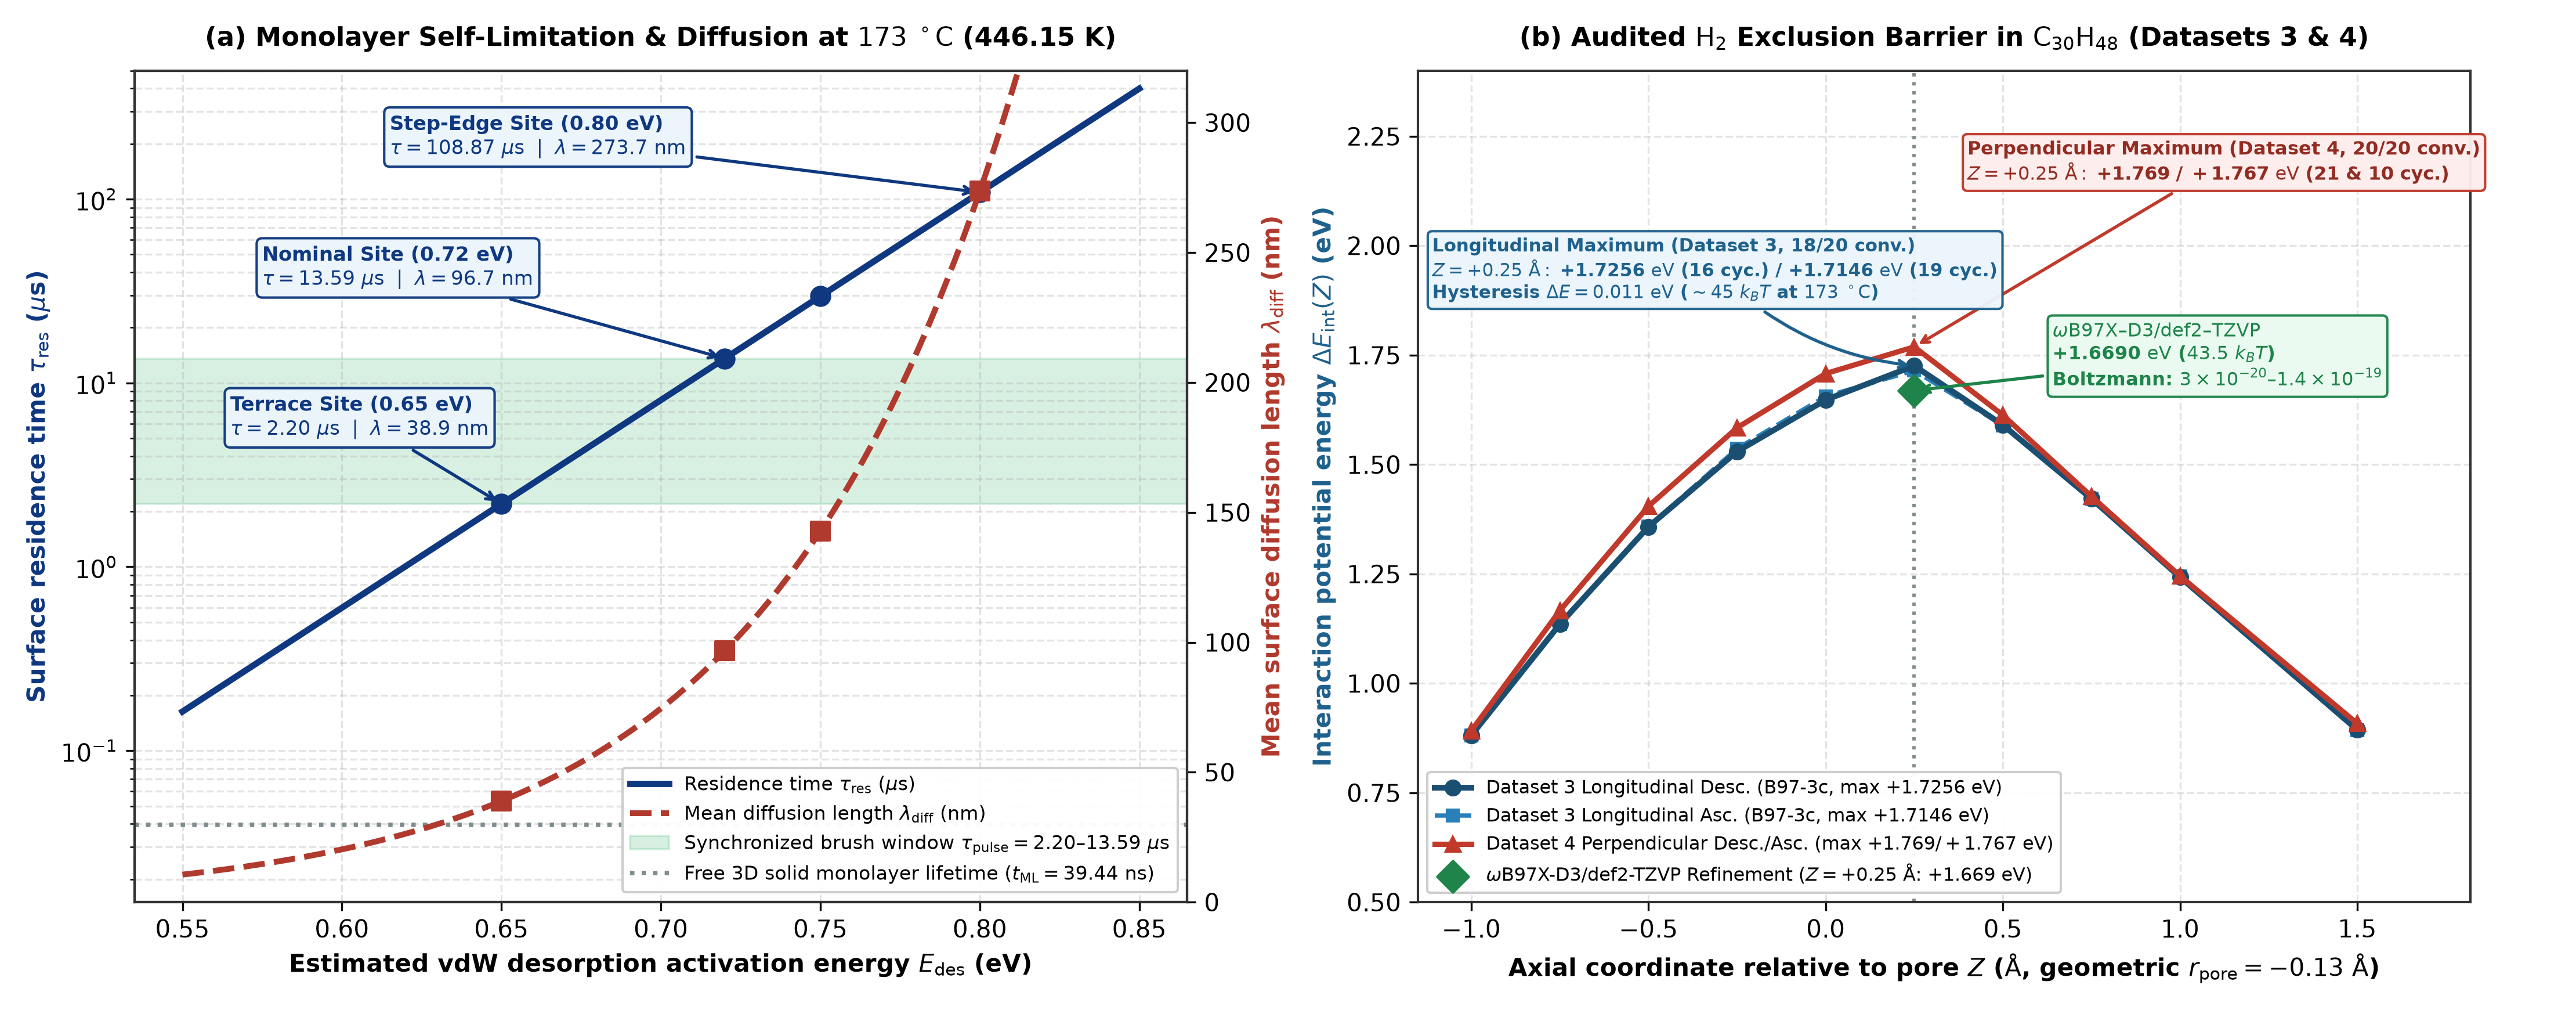
\includegraphics[width=0.98\textwidth]{fig1_thermodynamics_pore_barrier_173C_EN.png}
    \caption{\textbf{Surface self-limitation physics at $173\ ^\circ\text{C}$ and audited $\text{C}_{30}\text{H}_{48}$ quantum pore barrier (Datasets 3 and 4).} (a) Frenkel-Arrhenius residence time $\tau_{\text{res}}$ and surface diffusion length $\lambda_{\text{diff}}$ as functions of estimated vdW desorption activation energy $E_{\text{des}}$ at $446.15\text{ K}$, contrasted with the $39.44\text{ ns}$ evaporation of unconfined 3D solid and the synchronized VUV brush window ($\tau_{\text{pulse}} = 2.20\text{--}13.59\ \mu\text{s}$). (b) Audited adiabatic interaction potential profiles $\Delta E_{\text{int}}(Z)$ for $\text{H}_2$ traversing the three-adamantane pore ($\text{C}_{30}\text{H}_{48}$, $r_{\text{pore}} = -0.13\text{ \AA}$) in ORCA 6.1.1: Dataset 3 longitudinal ($\theta_Z = 5.82^\circ$, maximum at $Z = +0.25\text{ \AA}$ of $+1.7256\text{ eV}$ in $16$ cycles desc.\ and $+1.7146\text{ eV}$ in $19$ cycles asc.), Dataset 4 perpendicular ($\theta_Z = 95.60^\circ$, $+1.769 / +1.767\text{ eV}$), and $\omega\text{B97X-D3}$/def2-TZVP refinement ($+1.669\text{ eV}$).}
    \label{fig:termo_poro}
\end{figure*}

% ==============================================================================
% 4. THERMODYNAMICS AND MONOLAYER SELF-LIMITATION AT 173 °C
% ==============================================================================
\section{Thermodynamics of Adamantane and Monolayer Self-Limitation at $173\ ^\circ\text{C}$ ($446.15\text{ K}$)}

While early electron-beam experiments operated cryogenically ($100\text{ K} = -173\ ^\circ\text{C}$) \cite{Fu2025} to immobilize solid microcrystals of precursor, operating at $\mathbf{+173\ ^\circ\text{C}}$ ($\mathbf{446.15\text{ K}}$) shifts the system from solid-state radiolysis into an adsorption-diffusion-desorption controlled epitaxial regime. Adamantane undergoes a solid-solid phase transition from its low-temperature tetragonal phase ($\text{crII}$) to its face-centered cubic plastic crystal phase ($\text{crI}$, $Fm\bar{3}m$) between $169.31\text{ K}$ and $217.82\text{ K}$ ($\Delta_{\text{trs}}H^\circ_m = 3276 \pm 12\text{ J}\cdot\text{mol}^{-1}$), melting at $T_{\text{fus}} = 543.2\text{ K}$ ($270.05\ ^\circ\text{C}$, $\Delta_{\text{fus}}H^\circ_m = 13.96 \pm 0.28\text{ kJ}\cdot\text{mol}^{-1}$) \cite{Bazyleva2011}. At $446.15\text{ K}$, the molar heat capacity of the plastic phase $\text{crI}$, described by:
\begin{equation}
\begin{split}
C_{p,m}(\text{crI}) &= 50.80 + 0.1527\left(\frac{T}{\text{K}}\right) \\
&\quad + 1.052 \times 10^{-3}\left(\frac{T}{\text{K}}\right)^2\ \text{J}\cdot\text{K}^{-1}\cdot\text{mol}^{-1}
\end{split}
\end{equation}
reaches $C_{p,m} = 328.3\text{ J}\cdot\text{K}^{-1}\cdot\text{mol}^{-1}$, reflecting unhindered isotropic molecular rotation.

From the Clausius-Clapeyron relation ($\Delta_{\text{sub}}H_T \approx 59.8\text{--}60.0\text{ kJ}\cdot\text{mol}^{-1}$, $P_{\text{sat}}(298.15\text{ K}) \approx 1.3\text{--}1.5\text{ Pa}$), the saturation vapor pressure at $446.15\text{ K}$ rises to $P_{\text{sat}} = 4332.2\text{ Pa}$ ($32.49\text{ Torr}$, range $3991.2\text{--}4481.6\text{ Pa}$). Substituting $M_{\text{Ad}} = 136.23\text{ g}\cdot\text{mol}^{-1}$ ($m_{\text{Ad}} = 2.262 \times 10^{-25}\text{ kg}$) and $k_B T = 0.0384\text{ eV}$ into the Hertz-Knudsen sublimation rate:
\begin{equation}
\begin{split}
Z_{\text{evap}} &= \frac{P_{\text{sat}}}{\sqrt{2\pi m_{\text{Ad}} k_B T}} \\
&= 4.630 \times 10^{21}\ \text{molecules}\cdot\text{cm}^{-2}\cdot\text{s}^{-1}
\end{split}
\end{equation}
For a compact monolayer (ML) of adamantane ($d_{\text{mol}} \approx 0.74\text{ nm}$, molecular footprint $A_{\text{mol}} \approx 0.548\text{ nm}^2$, $\sigma_{\text{ML}} \approx 1.83 \times 10^{14}\text{ molec}\cdot\text{cm}^{-2}$), the evaporation lifetime of an unconfined solid monolayer at $173\ ^\circ\text{C}$ is just:
\begin{equation}
t_{\text{ML}} = \frac{\sigma_{\text{ML}}}{Z_{\text{evap}}} = 39.44\text{ ns}\ (0.04\ \mu\text{s})
\end{equation}

This volatility has an extraordinarily beneficial physical consequence: \textbf{it strictly prevents the parasitic condensation of 3D amorphous adamantane multilayers on the growth surface}. Surface population is intrinsically self-limited to a physisorbed sub-monolayer or monolayer, where van der Waals dispersion with the dense diamond substrate raises desorption energy to $E_{\text{des}} = 0.65\text{--}0.80\text{ eV}$ ($63\text{--}77\text{ kJ}\cdot\text{mol}^{-1}$). Applying the Frenkel-Arrhenius law ($\tau_{\text{res}} = \tau_0 \exp(E_{\text{des}}/k_B T)$ with attempt period $\tau_0 \approx 1.0 \times 10^{-13}\text{ s}$), the surface residence time at $173\ ^\circ\text{C}$ ranges from $\tau_{\text{res}} = 2.20\ \mu\text{s}$ on flat terraces ($0.65\text{ eV}$), to $13.59\ \mu\text{s}$ at nominal sites ($0.72\text{ eV}$), $29.66\ \mu\text{s}$ at $0.75\text{ eV}$, and $108.87\ \mu\text{s}$ along step edges ($0.80\text{ eV}$). Assuming hopping distance $a_{\text{hop}} = 0.5\text{ nm}$, attempt frequency $\nu_0 = 1.0 \times 10^{12}\text{ s}^{-1}$, and migration barrier $E_{\text{diff}} = 0.20\text{ eV}$, surface diffusivity is $D_s = \frac{1}{4}a_{\text{hop}}^2 \nu_0 \exp(-E_{\text{diff}}/k_B T) = 3.441 \times 10^{-6}\text{ cm}^2\cdot\text{s}^{-1}$, and the mean diffusion length before desorption ($\lambda_{\text{diff}} = \sqrt{2 D_s \tau_{\text{res}}}$) spans $38.91\text{ nm}$ to $273.72\text{ nm}$ ($96.71\text{ nm}$ nominal, Figure~\ref{fig:termo_poro}a and Table~\ref{tab:termo_173C}).

\begin{table*}[t]
\centering
\caption{\textbf{Thermodynamic and kinetic parameters of adamantane on diamond at $173\ ^\circ\text{C}$ ($446.15\text{ K}$).}}
\label{tab:termo_173C}
\setlength{\tabcolsep}{4pt}
\resizebox{\textwidth}{!}{%
\begin{tabular}{@{}llcll@{}}
\toprule
\textbf{Thermodynamic / Kinetic Parameter} & \textbf{Symbol} & \textbf{Value at $173\ ^\circ\text{C}$ ($446.15\text{ K}$)} & \textbf{Units} & \textbf{Physical Implication in DIET Process} \\ \midrule
Thermal energy of substrate & $k_B T$ & $0.0384$ & $\text{eV}$ & Rotational coupling without breaking $\text{C--C}$ bonds \\
Molar heat capacity ($\text{crI}$) & $C_{p,m}$ & $328.3$ & $\text{J}\cdot\text{K}^{-1}\cdot\text{mol}^{-1}$ & Plastic FCC phase with unhindered isotropic rotation \\
Standard sublimation enthalpy & $\Delta_{\text{sub}}H$ & $59.8\text{--}60.0$ & $\text{kJ}\cdot\text{mol}^{-1}$ & Low intermolecular van der Waals cohesion \\
Saturation vapor pressure & $P_{\text{sat}}$ & $4332.2\ (32.49)$ & $\text{Pa}\ (\text{Torr})$ & High volatility; prevents 3D amorphous condensation \\
Hertz-Knudsen evaporative flux & $Z_{\text{evap}}$ & $4.630 \times 10^{21}$ & $\text{molec}\cdot\text{cm}^{-2}\cdot\text{s}^{-1}$ & Instantaneous desorption of unbonded solid \\
Compact monolayer density & $\sigma_{\text{ML}}$ & $1.83 \times 10^{14}$ & $\text{molec}\cdot\text{cm}^{-2}$ & Close-packing with molecular footprint $A_{\text{mol}} = 0.548\text{ nm}^2$ \\
Lifetime of free $1\text{ ML}$ solid & $t_{\text{ML}}$ & $39.44$ & $\text{ns}$ & Suppresses bulk parasitic nucleation at $173\ ^\circ\text{C}$ \\
Minimum residence time ($0.65\text{ eV}$) & $\tau_{\text{res,min}}$ & $2.20$ & $\mu\text{s}$ & Lower bound on terraces $(100)\text{-}(2\times 1):\text{H}$ and $\{111\}\text{-}(1\times 1):\text{H}$ \\
Nominal residence time ($0.72\text{ eV}$) & $\tau_{\text{res,nom}}$ & $13.59$ & $\mu\text{s}$ & Nominal time window for brush photon capture \\
Maximum residence time ($0.80\text{ eV}$) & $\tau_{\text{res,max}}$ & $108.87$ & $\mu\text{s}$ & Prolonged trapping along step risers and active defects \\
Surface diffusion coefficient & $D_s$ & $3.441 \times 10^{-6}$ & $\text{cm}^2\cdot\text{s}^{-1}$ & High lateral mobility of physisorbed cages \\
Mean diffusion length ($0.65\text{--}0.80\text{ eV}$) & $\lambda_{\text{diff}}$ & $38.91\text{--}273.72$ & $\text{nm}$ & Centripetal feeding toward advancing step edges \\
Kinetic isotope effect ($\text{Ad-}h_{16}/\text{Ad-}d_{16}$) & $\text{KIE}$ & $2.0$ & Dimensionless & Confirms $\text{C--H}$ scission as rate-determining step (RDS) \\ \bottomrule
\end{tabular}%
}
\end{table*}

% ==============================================================================
% 5. DIET QUANTUM MECHANISM: E-BEAM (1.0 keV) VS VUV PHOTONS (6.49-10 eV)
% ==============================================================================
\section{Quantum Physics of the DIET Mechanism: Electron Beam ($1.0\text{ keV}$) vs.\ VUV Photons ($6.49\text{--}10.0\text{ eV}$)}

Selective $\text{C--H}$ activation proceeds through Desorption Induced by Electronic Transitions (DIET) via three channels \cite{Menzel1964,Avouris1989}: (i) \textbf{Menzel-Gomer-Redhead (MGR)}, involving $\sigma(\text{C--H}) \to \sigma^*(\text{C--H})$ promotion or repulsive Rydberg states ejecting neutral $\text{H}^\bullet$; (ii) \textbf{Knotek-Feibelman (KF)}, driven by inner-valence ionization and Auger decay to $2h/3h$ localized states expelling $\text{H}^+$; and (iii) \textbf{Dissociative Electron Attachment (DEA)} of slow secondary electrons ($1\text{--}20\text{ eV}$) into $\sigma^*(\text{C--H})$ forming a transient negative ion ($\text{TNI}$, $[\text{Ad}]^{\bullet-}$) that dissociates into $\text{Ad}^\bullet + \text{H}^-/\text{H}^\bullet$.

\subsection{Inelastic Transport and Secondary Cascades under a $1.0\text{ keV}$ Electron Beam}
In a diamond substrate ($\rho = 3.52\text{ g}\cdot\text{cm}^{-3}, Z=6, A=12.011\text{ g}\cdot\text{mol}^{-1}$), the Kanaya-Okayama range \cite{Kanaya1972}:
\begin{equation}
R_{\text{KO}} = \frac{0.0276\,A}{\rho\,Z^{0.89}} E_0^{1.67}\quad [\mu\text{m}]
\end{equation}
yields a penetration depth at $E_0 = 1.0\text{ keV}$ of $R_{\text{KO,diam}} = 19.12\text{ nm}$ ($51.55\text{ nm}$ in solid adamantane). Relativistic knock-on energy transfer to carbon nuclei is bounded by $T_{\text{max}} = 2 E_0 (E_0 + 2 m_e c^2)/(M_{\text{C}} c^2) = 0.1829\text{ eV}$, lying $191.4\times$ below the bulk vacancy displacement threshold of diamond ($E_d = 35.0\text{ eV}$). Electronic stopping power from the Bethe-Joy-Luo model ($I = 88.5 \pm 2.0\text{ eV}$) reaches $-\left.dE/ds\right|_{\text{diam}} = 3653.38\text{ eV}\cdot\text{nm}^{-1}$ ($365.34\text{ eV}\cdot\text{\AA}^{-1}$) compared to $-\left.dE/ds\right|_{\text{Ad}} = 1389.34\text{ eV}\cdot\text{nm}^{-1}$, with an inelastic mean free path $\lambda_{\text{IMFP}} \approx 2.0\text{ nm}$ ($\sim 14.7$ scattering events). Because the physisorbed monolayer at $173\ ^\circ\text{C}$ is only $\sim 0.74\text{ nm}$ thick, primary electrons deposit $<10\%$ of their energy in the precursor and $>90\%$ in the top $19.12\text{ nm}$ of the substrate.

On hydrogenated diamond surfaces exhibiting negative electron affinity (NEA), the secondary electron yield ($\text{SEY}, \delta = I_{\text{SE}}/I_p$) peaks at $E_0 \approx 1.0\text{ keV}$, releasing $\mathbf{\delta \approx 20}$ secondary electrons per incident primary ($\delta_{\text{max}} = 1.05$ in amorphous carbon). The total DIET activation rate under electron irradiation is:
\begin{equation}
\begin{split}
R_{\text{DIET,e}} &= J_e \Bigg[ \sigma_{\text{EII}}(1\text{ keV}) + \int_0^{50\text{ eV}} \frac{d\delta(E_s)}{dE_s} \\
&\quad \times \left(\sigma_{\text{ESD}}(E_s) + \sigma_{\text{DEA}}(E_s) + \sigma_{\text{EII}}(E_s)\right) dE_s \Bigg]
\end{split}
\end{equation}
where $\sigma_{\text{EII}}(1\text{ keV}) \approx 1.5\text{--}2.5 \times 10^{-16}\text{ cm}^2$ (peaking at $5.0\text{--}8.0 \times 10^{-16}\text{ cm}^2$ around $50\text{--}65\text{ eV}$), while $\sigma_{\text{ESD}}$ on hydrogenated diamond(100) scales from $5.0\text{ Mb}$ ($5 \times 10^{-18}\text{ cm}^2$) at $5\text{ eV}$ to $35.0\text{ Mb}$ at $37\text{ eV}$ \cite{Hoffman2002}. However, electron-beam processing exhibits three severe limitations (Figure~\ref{fig:diet_contraste}b): (1) high-energy primaries and secondary electrons $>20\text{--}70\text{ eV}$ fragment skeletal $\text{C--C}$ bonds ($m/z = 135 \to 93, 79, 67$), generating $8\text{--}15\%$ graphitic $sp^2$ defects; (2) electron-stimulated desorption of intact cages occurs ($\sigma_{\text{des,phys}} \sim 10^{-16}\text{ cm}^2$); and (3) positive hole accumulation $Q_1 = I_p t_c (\delta - 1)$ rapidly collapses the secondary yield to $\delta = 1$ at doses $D_{c1} = 0.2\text{ mC}\cdot\text{cm}^{-2}$ and $D_{c2} = 2.0\text{ mC}\cdot\text{cm}^{-2}$, extinguishing the NEA state.

\begin{figure*}[t]
    \centering
    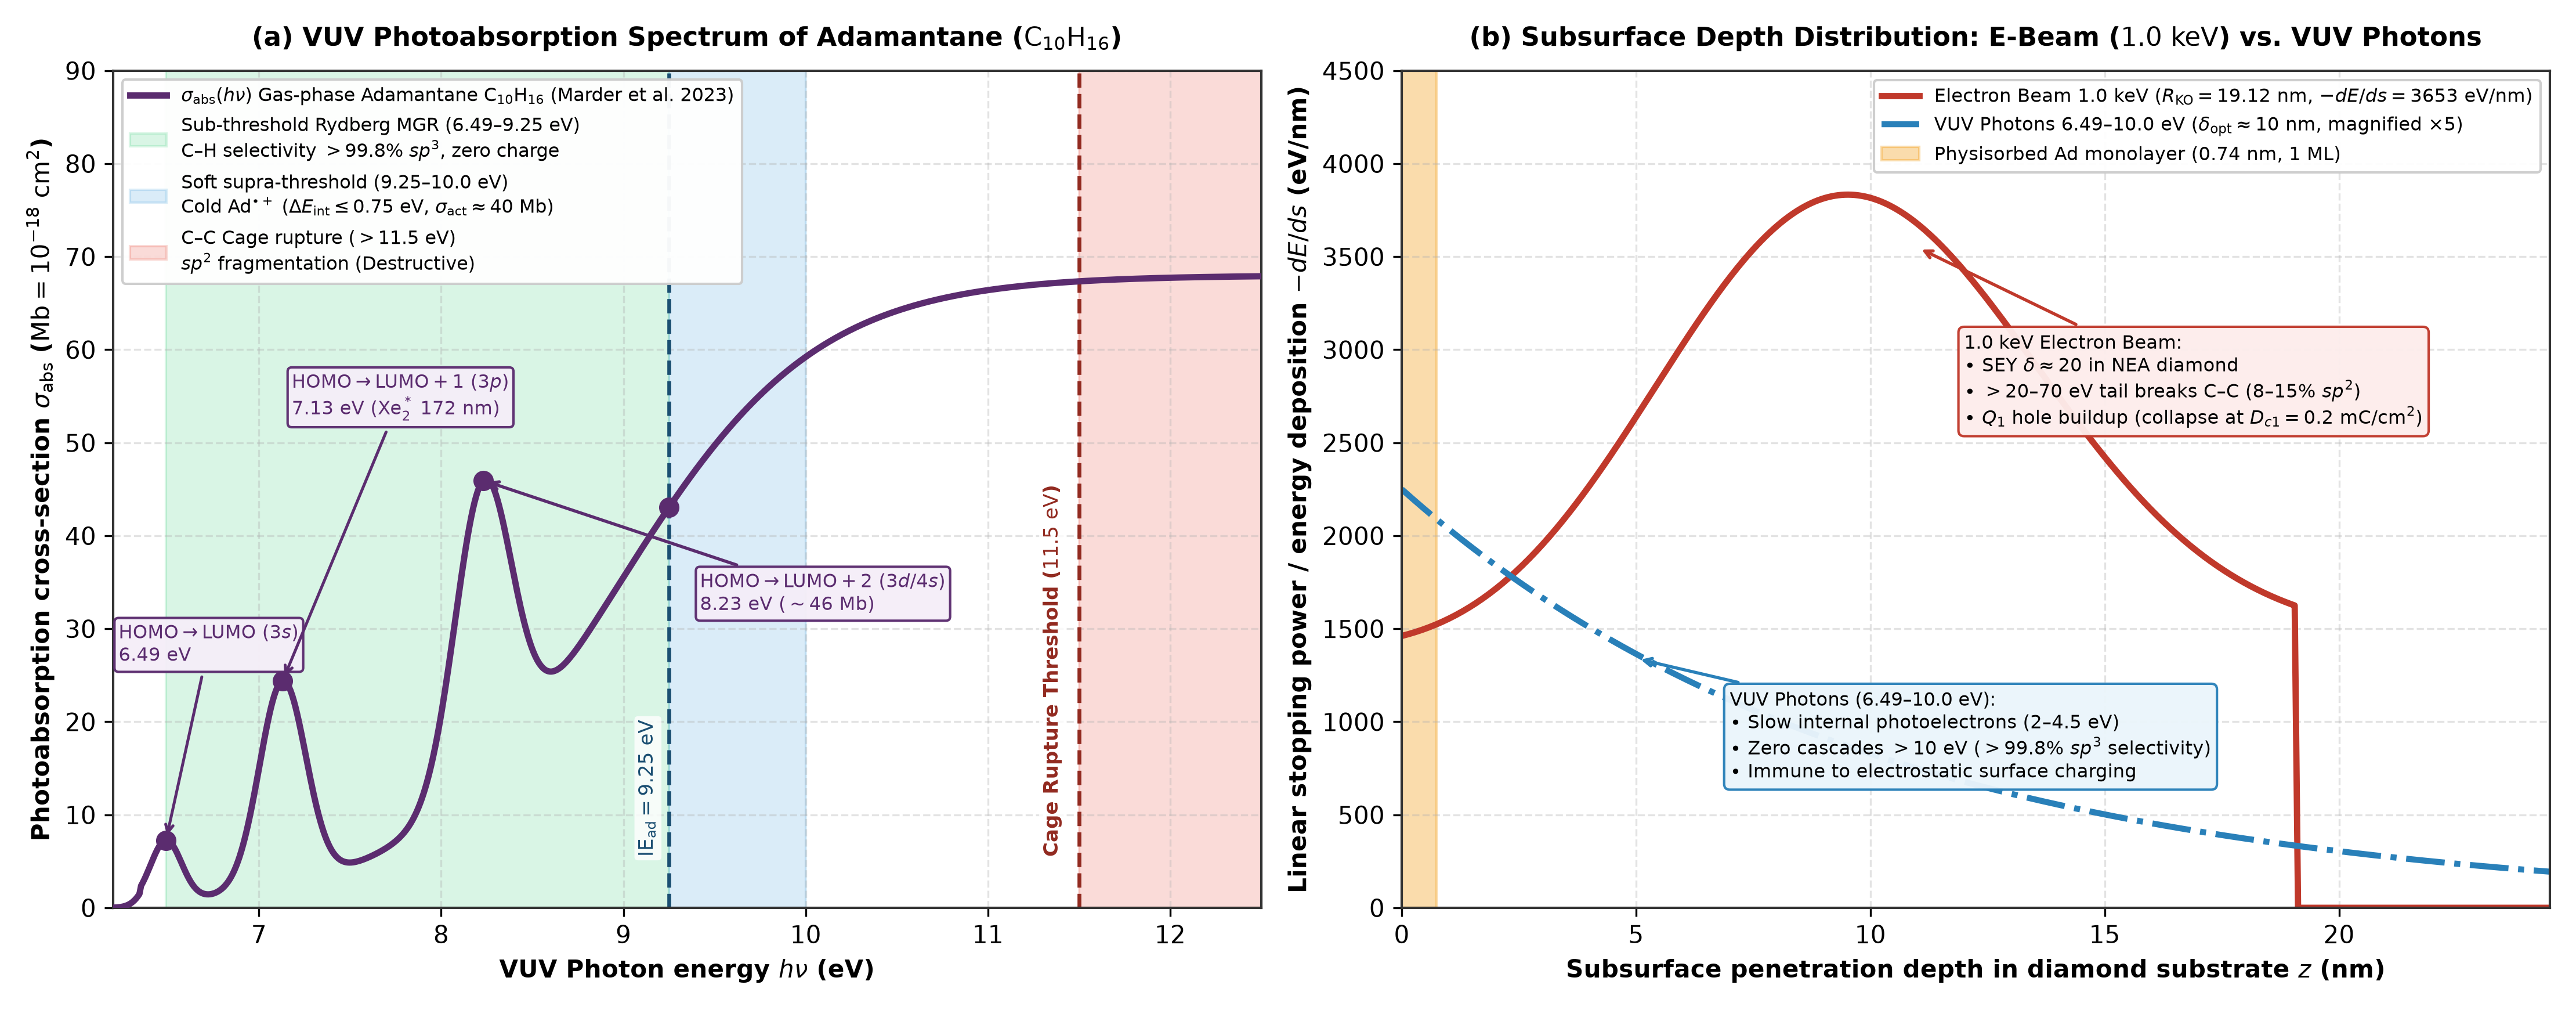
\includegraphics[width=0.98\textwidth]{fig2_diet_ebeam_vs_vuv_contrast_EN.png}
    \caption{\textbf{Quantum-physical contrast between VUV photon excitation ($6.49\text{--}10.0\text{ eV}$) and electron beam irradiation ($1.0\text{ keV}$).} (a) Absolute gas-phase VUV photoabsorption cross-section $\sigma_{\text{abs}}(h\nu)$ of adamantane ($\text{C}_{10}\text{H}_{16}$, Marder et al. 2023 \cite{Marder2023}), highlighting the sub-threshold cage Rydberg transitions at $6.49\text{ eV}$ ($\text{HOMO}\to\text{LUMO}$), $7.13\text{ eV}$ ($\text{HOMO}\to\text{LUMO}+1$, matching $\text{Xe}_2^*$ excimer emission at $172\text{ nm}$), and $8.23\text{ eV}$ ($\text{HOMO}\to\text{LUMO}+2$, $\sim 46\text{ Mb}$), alongside the soft supra-threshold window ($9.25\text{--}10.0\text{ eV}$) below the $\text{C--C}$ cage rupture threshold ($>11.5\text{ eV}$). (b) Subsurface energy deposition profile in diamond: Kanaya-Okayama collisional cascade at $1.0\text{ keV}$ ($R_{\text{KO}} = 19.12\text{ nm}$) versus clean optical absorption of VUV photons ($\delta_{\text{opt}} \approx 8\text{--}15\text{ nm}$, nominal profile at $\delta_{\text{opt}} = 10\text{ nm}$).}
    \label{fig:diet_contraste}
\end{figure*}

\subsection{Selective Resonant Excitation of Adamantane via VUV Photons ($6.49\text{--}10.0\text{ eV}$)}
VUV radiation spanning $6.49\text{--}10.0\text{ eV}$ ($\lambda = 191.0\text{--}124.0\text{ nm}$) eliminates energetic collisional cascades, partitioning naturally into two regimes bounded by the adiabatic ionization energy of adamantane ($\text{IE}_{\text{ad}} = 9.25\text{ eV}$, vertical $9.56\text{ eV}$ \cite{Landt2009,Marder2023}, Figure~\ref{fig:diet_contraste}a and Table~\ref{tab:ebeam_vs_vuv}):
\begin{enumerate}
    \item \textbf{Sub-Threshold Resonant Predissociation Regime ($6.49 \le h\nu < 9.25\text{ eV}$):} Direct photoionization is energetically forbidden. High-resolution gas-phase synchrotron spectroscopy by Marder et al. (2023) \cite{Marder2023} and Landt et al. (2009) \cite{Landt2009} demonstrates that adamantane ($\text{C}_{10}\text{H}_{16}$) exhibits three distinct Rydberg transitions originating from the $\text{HOMO}$ ($2t_2$) into cage-localized states: the optical absorption onset $\text{HOMO}\to\text{LUMO}$ ($3s \leftarrow 2t_2$) at $\mathbf{6.49\text{ eV}}$, the $\text{HOMO}\to\text{LUMO}+1$ ($3p \leftarrow 2t_2$) band at $\mathbf{7.13\text{ eV}}$ ($\sigma_{\text{abs}} \approx 24\text{ Mb}$, directly accessible using xenon excimer sources $\text{Xe}_2^*$ at $172\text{ nm} \equiv 7.21\text{ eV}$), and the prominent $\text{HOMO}\to\text{LUMO}+2$ ($3d/4s \leftarrow 2t_2$) band at $\mathbf{8.23\text{ eV}}$ ($\sigma_{\text{abs}} \approx 46\text{ Mb} = 4.6 \times 10^{-17}\text{ cm}^2$). These cage Rydberg states of tetrahedral $T_d$ adamantane contrast with the isolated cyclohexane ($\text{C}_6\text{H}_{12}$) resonance at $8.486\text{ eV}$ ($33.96\text{ Mb}$): fusing four chair rings shifts the Rydberg onset lower and concentrates oscillator strength over $16$ $\text{C--H}$ bonds. Vibronic coupling to repulsive $\sigma^*(\text{C--H})$ coordinates drives homolytic MGR dissociation ($\text{Ad}^* \to \text{Ad}^\bullet + \text{H}^\bullet$) well below the double $\text{C--C}$ cleavage threshold ($>11.5\text{--}12.0\text{ eV}$), yielding an estimated primary channel selectivity $>99.8\%\ sp^3$.
    \item \textbf{Soft Photoionization and Internal Photoemission Regime ($9.25 \le h\nu \le 10.0\text{ eV}$):} This channel enables direct photoionization ($\text{Ad} + h\nu \to \text{Ad}^{\bullet+} + e^-$, $\sigma_{\text{abs}} \approx 55\text{--}65\text{ Mb}$), imparting an internal excess energy to the radical cation of at most $\Delta E_{\text{int}} = h\nu - \text{IE}_{\text{ad}} \le 0.75\text{ eV}$. The resulting Jahn-Teller distortion ($T_d \to C_{3v}$) selectively weakens the apical $\text{C--H}$ bond without causing cage fragmentation. Simultaneously, photons absorbed in the topmost $\delta_{\text{opt}} \approx 8\text{--}15\text{ nm}$ of the diamond substrate ($10\text{--}15\text{ nm}$ sub-threshold, $8\text{--}12\text{ nm}$ supra-threshold, nominal $\delta_{\text{opt}} = 10\text{ nm}$, bandgap $E_g = 5.47\text{ eV}$) inject slow internal photoelectrons ($E_{\text{kin}} \approx 2\text{--}4.5\text{ eV}$) that populate surface $\sigma^*(\text{C--H})$ states ($\sigma_{\text{PSD}} \approx 5\text{ Mb}$) without creating hot carriers or trapped charge.
\end{enumerate}

\begin{table*}[t]
\centering
\caption{\textbf{Physical and mechanistic comparison between a $1.0\text{ keV}$ Electron Beam and VUV Photons in Adamantane ($6.49\text{--}10.0\text{ eV}$).}}
\label{tab:ebeam_vs_vuv}
\setlength{\tabcolsep}{4pt}
\resizebox{\textwidth}{!}{%
\begin{tabular}{@{}p{3.6cm}p{4.3cm}p{4.3cm}p{4.3cm}@{}}
\toprule
\textbf{Physical / Mechanistic Parameter} & \textbf{Electron Beam ($1.0\text{ keV}$)} & \textbf{Sub-Threshold VUV Photons ($6.49\text{--}9.25\text{ eV}$)} & \textbf{Supra-Threshold VUV Photons ($9.25\text{--}10.0\text{ eV}$)} \\ \midrule
Primary excitation channel & Impact ionization + SE cascade ($1\text{--}50\text{ eV}$) & $T_d$ cage Rydberg states: $6.49\text{ eV}$ ($3s$), $7.13\text{ eV}$ ($3p$), and $8.23\text{ eV}$ ($3d/4s$) (MGR) & Soft photoionization (Jahn-Teller $\text{Ad}^{\bullet+}$) + internal photoemission \\ \midrule
Cross-section in precursor ($\sigma$) & $\sigma_{\text{EII}}(1\text{ keV}) \approx 1.5\text{--}2.5 \times 10^{-16}\text{ cm}^2$ (peak $5\text{--}8 \times 10^{-16}\text{ cm}^2$) & $\sigma_{\text{abs}} \approx 24\text{ Mb}$ ($7.13\text{ eV}$) to $\mathbf{\sim 46\text{ Mb}}$ ($8.23\text{ eV}$) \cite{Marder2023} & $\sigma_{\text{abs}} \approx 55\text{--}65\text{ Mb}$ ($\sigma_{\text{DIET}}^{\text{act}} = \sigma_{\text{abs}}\Phi_{\text{DIET}} \approx \mathbf{40\text{ Mb}}$) \\ \midrule
Substrate $\text{C--H}$ cross-section & $\sigma_{\text{ESD}}(5\text{ eV}) = 5\text{ Mb}$; $\sigma_{\text{ESD}}(37\text{ eV}) = 35\text{ Mb}$ & Internal photoemission ($1.0\text{--}3.7\text{ eV}$, $\sigma_{\text{PSD}} \sim 1\text{ Mb}$) & Internal photoemission into $\sigma^*(\text{C--H})$ ($\sigma_{\text{PSD}} \approx 5\text{ Mb}$) \\ \midrule
Penetration depth in diamond & $R_{\text{KO}} = 19.12\text{ nm}$ ($\lambda_{\text{IMFP}} \approx 2.0\text{ nm}$) & Optical attenuation length $\delta_{\text{opt}} \approx 10\text{--}15\text{ nm}$ & Optical attenuation length $\delta_{\text{opt}} \approx 8\text{--}12\text{ nm}$ \\ \midrule
Stopping power / deposition & $3653.4\text{ eV}\cdot\text{nm}^{-1}$ (diam.); $1389.3\text{ eV}\cdot\text{nm}^{-1}$ (Ad) & Discrete quantum absorption ($6.49\text{--}9.25\text{ eV}$ per photon) & Discrete quantum absorption ($9.25\text{--}10.0\text{ eV}$ per photon) \\ \midrule
Secondary yield ($\text{SEY}, \delta$) & $\delta \approx 20$ in NEA diamond ($\delta \approx 1.05$ in a-C) & $\delta \ll 0.1$ (sub-vacuum or thermal electrons) & $\delta \approx 0.1\text{--}0.5$ (slow photoelectrons $<4.5\text{ eV}$) \\ \midrule
Theoretical $\text{C--H}$ vs $\text{C--C}$ selectivity & Moderate ($85\text{--}92\%$); $>20\text{ eV}$ tail causes $sp^2$ damage & \textbf{Ultra-high estimated ($>99.8\%$)}; below cage rupture & \textbf{Very high estimated ($>99.0\%$)}; cold $\text{Ad}^{\bullet+}$ ($\Delta E_{\text{int}} \le 0.75\text{ eV}$) \\ \midrule
Charge buildup and degradation & Severe hole trapping ($D_{c1}=0.2\text{ mC}\cdot\text{cm}^{-2}$), loss of NEA & \textbf{Negligible to zero}; predominantly neutral process & \textbf{Low}; easily neutralized in $p$-type substrates \\ \midrule
Diffraction-limited resolution & Sub-nanometer to nanometer ($\sim 1\text{--}5\text{ nm}$) & Diffraction-limited ($80\text{--}150\text{ nm}$) or near-field & Diffraction-limited ($65\text{--}120\text{ nm}$) or plasmonic mask \\ \bottomrule
\end{tabular}%
}
\end{table*}

% ==============================================================================
% 6. SPATIOTEMPORAL KINETICS: SYNCHRONIZED BRUSH VS FLOOD MODE
% ==============================================================================
\section{Spatiotemporal Kinetics: Synchronized Brush vs.\ Flood Mode}

The interplay between DIET activation and surface kinetics at $173\ ^\circ\text{C}$ ($446.15\text{ K}$) is governed by the coupled reaction-diffusion-desorption partial differential equations for physisorbed adamantane coverage $\theta_{\text{Ad}}(\mathbf{r},t)$ and activated radical density $\theta_{\text{Ad}^\bullet}(\mathbf{r},t)$:
\begin{equation}
\begin{split}
\frac{\partial \theta_{\text{Ad}}(\mathbf{r},t)}{\partial t} &= F_{\text{dos}}\left(1 - \theta_{\text{Ad}} - \theta_{\text{Ad}^\bullet}\right) - \frac{\theta_{\text{Ad}}}{\tau_{\text{res}}} \\
&\quad + D_s \nabla^2 \theta_{\text{Ad}} - \left(\sigma_{\text{DIET}}^{\text{act}} + \sigma_{\text{DIET}}^{\text{des}}\right) J(\mathbf{r},t)\,\theta_{\text{Ad}}
\end{split}
\end{equation}
\begin{equation}
\begin{split}
\frac{\partial \theta_{\text{Ad}^\bullet}(\mathbf{r},t)}{\partial t} &= \sigma_{\text{DIET}}^{\text{act}}\,J(\mathbf{r},t)\,\theta_{\text{Ad}} - k_{\text{epi}}\,\theta_{\text{Ad}^\bullet} N_{\text{step}}(\mathbf{r}) \\
&\quad - k_{\text{nuc}}\,\theta_{\text{Ad}^\bullet}^2 - \sigma_{\text{damage}}\,J(\mathbf{r},t)\,\theta_{\text{Ad}^\bullet}
\end{split}
\end{equation}
where $\sigma_{\text{DIET}}^{\text{act}} = \sigma_{\text{abs}}(h\nu)\,\Phi_{\text{DIET}}$ is the effective $\text{C--H}$ scission cross-section (nominal design value $\sigma_{\text{DIET}}^{\text{act}} = \mathbf{4.0 \times 10^{-17}\text{ cm}^2} \equiv 40\text{ Mb}$, corresponding to $\sigma_{\text{abs}} \approx 46\text{--}65\text{ Mb}$ across $8.23\text{--}9.6\text{ eV}$ \cite{Marder2023} and substrate-assisted quantum yield $\Phi_{\text{DIET}} \approx 0.62\text{--}0.85$). The dynamical behavior is governed by the \textbf{DIET Damköhler Number} ($\text{Da}_{\text{DIET}}$) and the \textbf{Scanning Péclet Number} ($\text{Pe}_{\text{scan}}$):
\begin{equation}
\begin{split}
\text{Da}_{\text{DIET}} &= \frac{\tau_{\text{res}}}{\tau_{\text{act}}} = \sigma_{\text{DIET}}^{\text{act}}\,J(\mathbf{r},t)\,\tau_{\text{res}}, \\
\text{Pe}_{\text{scan}} &= \frac{v_{\text{scan}}\,w_b}{D_s}
\end{split}
\end{equation}

\subsection{Kinetic and Structural Breakdown of the Simultaneous (Flood) Mode}
Under uncollimated flood irradiation (flood gun with $I_p \approx 75\text{--}150\ \mu\text{A}$ over $5\text{ cm}^2$, $J_{\text{flood}} \approx 1.0\text{--}2.0 \times 10^{14}\text{ e}^-\cdot\text{cm}^{-2}\cdot\text{s}^{-1}$; or flood VUV lamp with $10\text{--}50\text{ mW}\cdot\text{cm}^{-2}$, $J_{\text{flood}} \approx 0.7\text{--}3.0 \times 10^{16}\text{ photons}\cdot\text{cm}^{-2}\cdot\text{s}^{-1}$), the characteristic activation time for $\sigma_{\text{DIET}}^{\text{act}} = 4.0 \times 10^{-17}\text{ cm}^2$ is $\tau_{\text{act,flood}} = (\sigma_{\text{DIET}}^{\text{act}} J_{\text{flood}})^{-1} \approx \mathbf{0.83\text{--}3.57\text{ s}}$ in VUV ($\sim 0.1\text{--}10\text{ s}$ for electrons). Comparing this to the nominal surface residence time $\tau_{\text{res,nom}} = 13.59\ \mu\text{s}$ at $173\ ^\circ\text{C}$:
\begin{equation}
\begin{split}
\text{Da}_{\text{DIET,flood}} &= \frac{\tau_{\text{res,nom}}}{\tau_{\text{act,flood}}} \\
&\approx 3.8 \times 10^{-6}\text{ to }1.6 \times 10^{-5}\text{ (VUV)} \\
&\quad \left[\text{up to }10^{-4}\text{ in E-Beam}\right] \ll 1
\end{split}
\end{equation}
More than $\mathbf{99.998\%}$ of adamantane molecules desorb thermally prior to electronic excitation (Figure~\ref{fig:pincel_piramide}a). In addition, flood mode triggers four coupled pathologies: (1) random multi-site nucleation producing incommensurate islands that coalesce into fivefold twinned nanodiamonds; (2) central diffusive depletion ($\nabla\theta_{\text{Ad}} \approx 0$, suppressing the Laplacian $D_s \nabla^2 \theta_{\text{Ad}}$); (3) continuous over-irradiation and amorphization of newly anchored nuclei (reaching critical dose $D_{c1} = 0.2\text{ mC}\cdot\text{cm}^{-2}$ in $6.7\text{ s}$ at $150\ \mu\text{A}$, or $13.3\text{ s}$ at $75\ \mu\text{A}$); and (4) simultaneous release of hydrogen across large areas, trapping sub-surface $\text{H}_2$ bubbles that cause blister delamination.

\begin{figure*}[t]
    \centering
    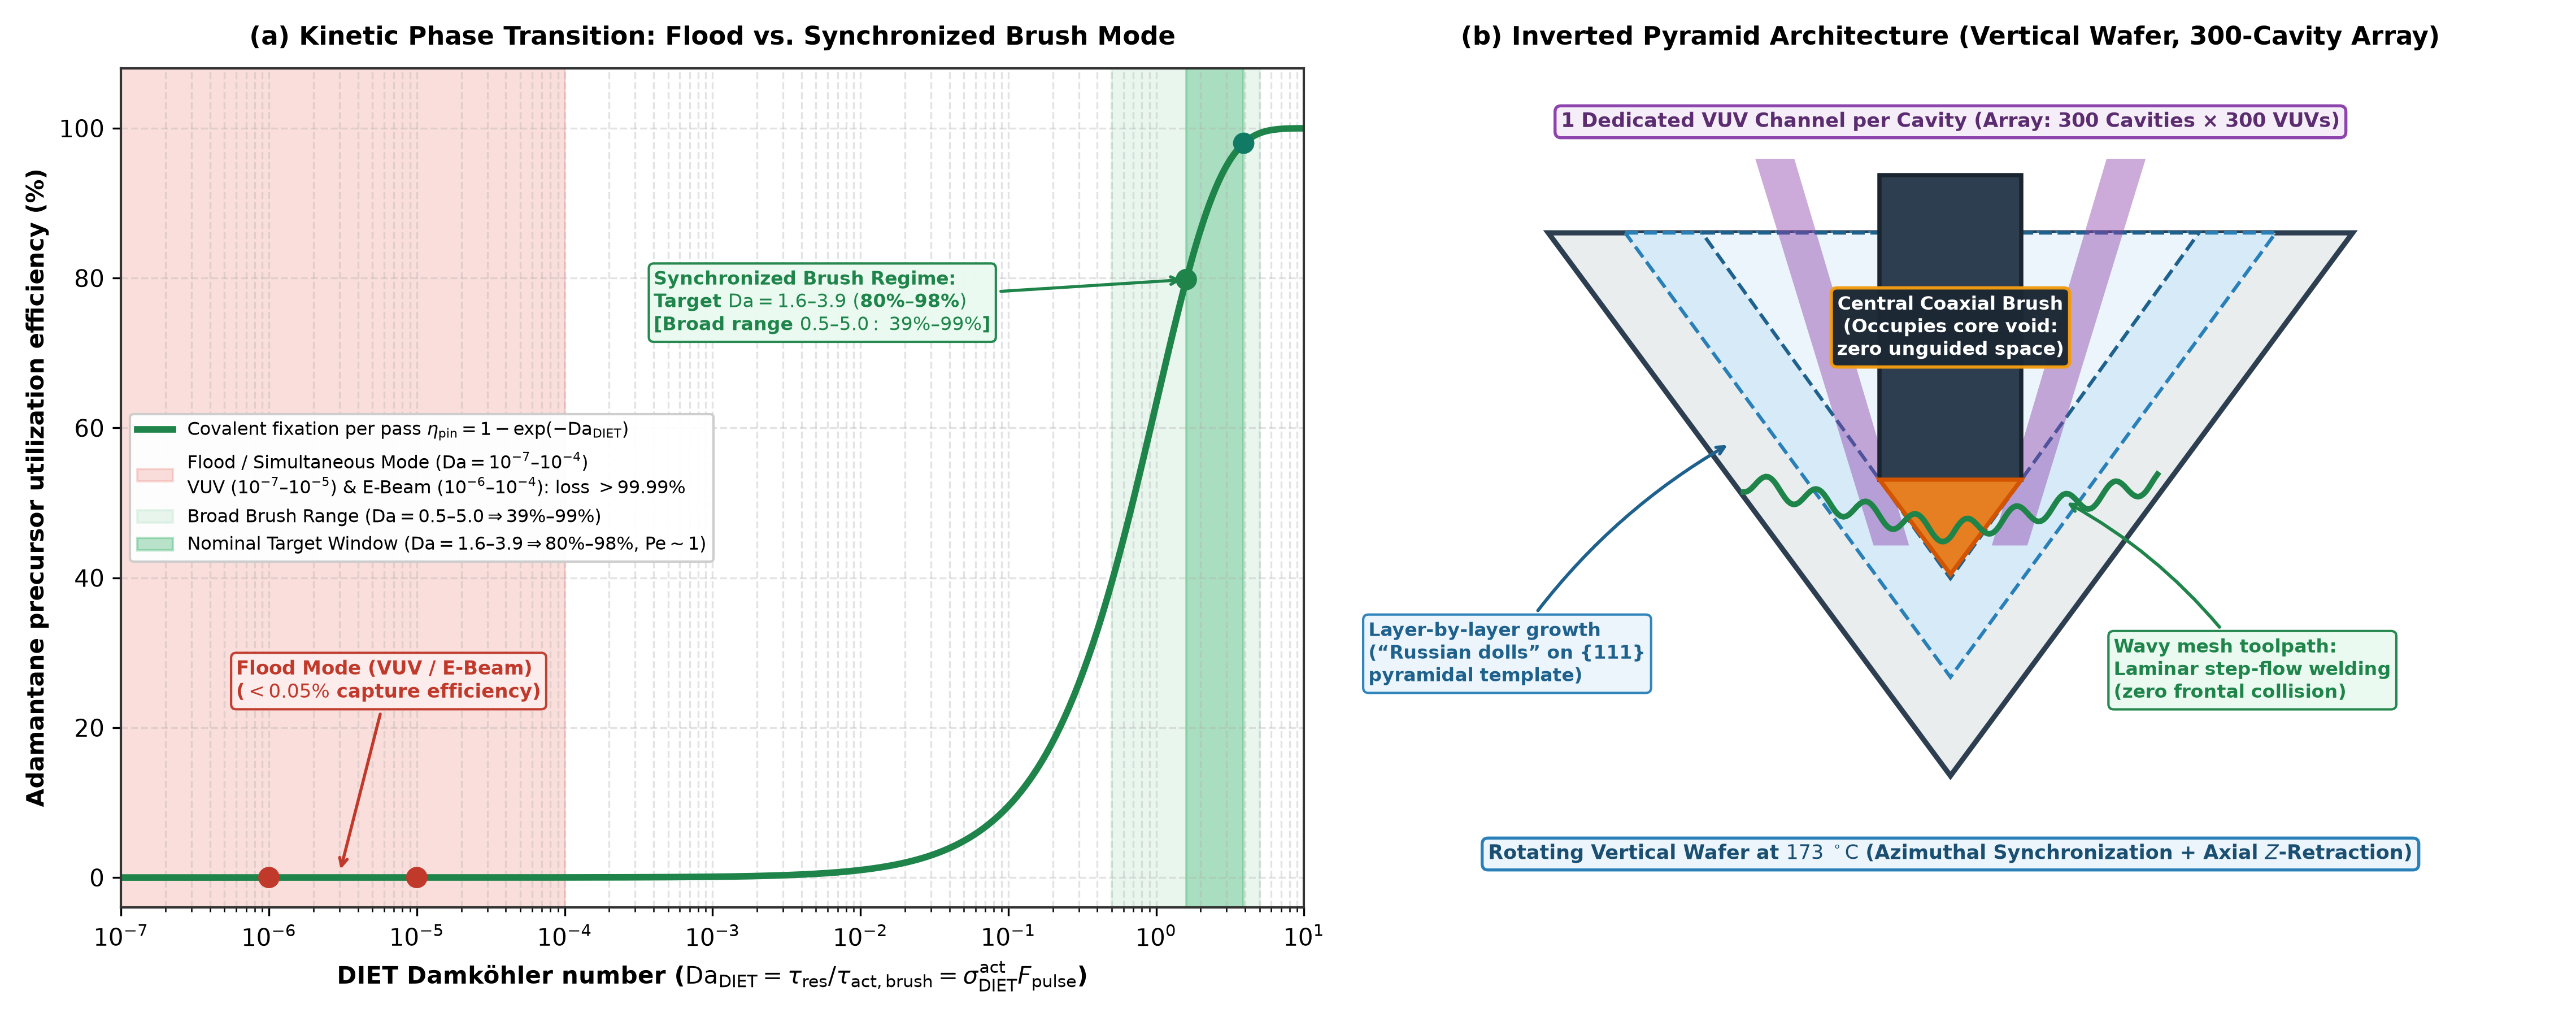
\includegraphics[width=0.98\textwidth]{fig3_brush_kinetics_inverted_pyramid_EN.png}
    \caption{\textbf{Synchronized brush kinetics and inverted pyramid epitaxy architecture.} (a) Covalent capture efficiency per pass ($\eta_{\text{pin}} = 1 - \exp(-\text{Da}_{\text{DIET}})$) versus DIET Damköhler number $\text{Da}_{\text{DIET}}$, contrasting flood mode ($\text{Da} \sim 10^{-7}\text{--}10^{-5}$ in VUV and $10^{-6}\text{--}10^{-4}$ in E-Beam, efficiency $<0.05\%$) with the synchronized brush regime (broad band $\text{Da} = 0.5\text{--}5.0 \implies 39\%\text{--}99\%$, nominal target window $\text{Da} = 1.6\text{--}3.9 \implies 80\%\text{--}98\%$). (b) Schematic of the Brush-VUV-Inverted Pyramid architecture: the central brush occupies the inner core, depositing undulating toolpaths (\textit{laminar welding} without frontal collision) in ``Russian dolls'' fashion under local VUV illumination on a rotating vertical wafer array scaled to $300$ cavities with $300$ independent VUV channels.}
    \label{fig:pincel_piramide}
\end{figure*}

\subsection{Directed Step-Flow Dynamics in Progressive Mode (Synchronized Brush)}
By focusing optical power of $P_{\text{channel}} \approx 80\text{--}200\text{ nW}$ per VUV micro-beam ($5.8 \times 10^{10}$ to $1.4 \times 10^{11}\text{ photons}\cdot\text{s}^{-1}$) into a nanometric spot of width $w_b \approx 40\text{--}100\text{ nm}$ ($50\text{ nm}$ nominal, focal area $A_{\text{brush}} = \frac{\pi}{4}w_b^2 \approx 1.96 \times 10^{-11}\text{ cm}^2$), local instantaneous photon flux reaches $J_{\text{brush}} = 2.94 \times 10^{21}\text{ to }7.18 \times 10^{21}\text{ photons}\cdot\text{cm}^{-2}\cdot\text{s}^{-1}$ in the target window ($9.20 \times 10^{20}\text{ to }9.19 \times 10^{21}\text{ photons}\cdot\text{cm}^{-2}\cdot\text{s}^{-1}$ broad band). For $\sigma_{\text{DIET}}^{\text{act}} = 4.0 \times 10^{-17}\text{ cm}^2$, the characteristic activation time drops to $\tau_{\text{act,brush}} = (\sigma_{\text{DIET}}^{\text{act}} J_{\text{brush}})^{-1} = 3.48\text{--}8.50\ \mu\text{s}$ ($2.72\text{--}27.18\ \mu\text{s}$ broad band), unlocking three precision couplings (Table~\ref{tab:cuatro_modos}):
\begin{enumerate}
    \item \textbf{Pulse Duration Matching ($\tau_{\text{pulse}} \equiv \tau_{\text{dwell}} = \tau_{\text{res}}$) and Temporal Coupling ($\text{Da}_{\text{DIET,brush}} \ge 1$):} Each surface site receives an exposure window matched to the physisorption residence time at $173\ ^\circ\text{C}$: $\tau_{\text{pulse}} \equiv \tau_{\text{dwell}} = w_b / v_{\text{scan}} = \mathbf{13.59\ \mu\text{s}}$ at nominal sites ($0.72\text{ eV}$, spanning $2.20\text{--}13.59\ \mu\text{s}$ from terraces to nominal sites and up to $108.87\ \mu\text{s}$ at step edges, with the full residence window encompassing $2.20\text{--}108.87\ \mu\text{s}$), delivering an integrated fluence per pass of $F_{\text{pulse}} = J_{\text{brush}}\tau_{\text{pulse}} = 4.00 \times 10^{16}\text{ to }9.76 \times 10^{16}\text{ photons}\cdot\text{cm}^{-2}$. Consequently, the local Damköhler number ($\text{Da}_{\text{DIET,brush}} = \tau_{\text{pulse}}/\tau_{\text{act,brush}} = \sigma_{\text{DIET}}^{\text{act}} F_{\text{pulse}}$) settles into the nominal target range \textbf{$\text{Da}_{\text{DIET,brush}} = 1.60$ to $3.91$}, yielding a covalent fixation efficiency per pass of $\eta_{\text{pin}} = 1 - \exp(-\text{Da}_{\text{DIET,brush}}) = \mathbf{80.0\%\text{ to }98.0\%}$ ($39.3\%\text{ to }99.3\%$ over the extended band $\text{Da}_{\text{DIET,brush}} = 0.50\text{--}5.00$).
    \item \textbf{Centripetal Diffusive Feeding ($w_b \lesssim \lambda_{\text{diff}}$, $\text{Pe}_{\text{scan}} \approx 1$):} Because $A_{\text{brush}}/A_{\text{sub}} < 10^{-5}$ and $w_b = 50\text{ nm} \lesssim \lambda_{\text{diff}} = 96.71\text{ nm}$ ($v_{\text{diff}} \approx 2 D_s / w_b = 1.38\text{ cm}\cdot\text{s}^{-1}$), scanning at $v_{\text{scan}} \approx 0.37\text{--}2.3\text{ cm}\cdot\text{s}^{-1}$ maintains \textbf{$\text{Pe}_{\text{scan}} = v_{\text{scan}} w_b / D_s \approx 0.54\text{--}3.3 \sim \mathcal{O}(1)$}. The Laplacian term $D_s \nabla^2 \theta_{\text{Ad}}$ draws precursor from adjacent non-illuminated surface reservoirs toward $\langle 110 \rangle$ step edges on both $\{111\}\text{-}(1\times 1):\text{H}$ pyramidal facets and $(100)/(001)\text{-}(2\times 1):\text{H}$ reference terraces (\textit{step-flow epitaxy}), preventing random island nucleation.
    \item \textbf{Dark Refresh Window ($\tau_{\text{refresh}} \approx 1\text{--}50\text{ ms}$, Duty Cycle $\tau_{\text{pulse}}/\tau_{\text{refresh}} \approx 2.7 \times 10^{-4}\text{ to }1.4 \times 10^{-2}$):} Between successive passes over a given coordinate ($f_{\text{rep}} = 20\text{ Hz to }1\text{ kHz}$), the surface rests in the dark for $\tau_{\text{refresh}} = 1\text{--}50\text{ ms}$ (enforcing a low duty cycle $\le 10^{-3}$ for $\tau_{\text{refresh}} \ge 13.6\text{ ms}$): physisorbed coverage replenishes in $\sim 13.6\ \mu\text{s}$, byproduct $\text{H}_2$ desorbs unimpeded into the Turbo-NEG UHV environment, and any residual excitation neutralizes.
\end{enumerate}

\begin{table*}[t]
\centering
\caption{\textbf{Theoretical performance comparison across the four spatiotemporal and DIET excitation modes at $173\ ^\circ\text{C}$.}}
\label{tab:cuatro_modos}
\setlength{\tabcolsep}{4pt}
\resizebox{\textwidth}{!}{%
\begin{tabular}{@{}p{2.9cm}p{3.3cm}p{3.3cm}p{3.5cm}p{3.5cm}@{}}
\toprule
\textbf{Performance Dimension} & \textbf{Flood Mode + E-Beam ($1.0\text{ keV}$)} & \textbf{Flood Mode + VUV ($6.49\text{--}10\text{ eV}$)} & \textbf{Synchronized Brush + E-Beam ($1.0\text{ keV}$)} & \textbf{Synchronized Brush + VUV ($6.49\text{--}10\text{ eV}$)} \\ \midrule
Damköhler Number ($\text{Da}_{\text{DIET}}$) & $10^{-6}\text{--}10^{-4}$ (Desorption dominated) & $10^{-7}\text{--}10^{-5}$ (Desorption dominated) & $1.1\text{--}2.5$ (Focused capture with electron-stimulated desorption) & \textbf{$1.6\text{--}3.9$ target} ($0.5\text{--}5.0$ broad band) \\ \midrule
Fixation efficiency ($\eta_{\text{pin}}$) & $< 0.05\%$ (Massive sublimation loss) & $< 0.01\%$ (Sublimation exceeds photoactivation) & $65\%\text{--}92\%$ (Diffusively fed by $\lambda_{\text{diff}}$) & $\mathbf{80\%\text{--}98\%\text{ target}}$ ($39\%\text{--}99\%$ in $\text{Da}=0.5\text{--}5.0$) \\ \midrule
Growth mode & Random 3D/2D island nucleation & Dispersed 2D nucleation (flux limited) & Directional step-flow epitaxy & \textbf{Self-limited coherent step-flow epitaxy} \\ \midrule
Estimated film morphology & Polycrystalline, fivefold twins + $sp^2$ & Nanocrystalline, high $sp^3$ purity but multi-domain & Monocrystalline / nanopatterns; $sp^2$ traces ($<2\%$) & \textbf{Monocrystalline ($>99.8\%\ sp^3$ est.), twin-free} \\ \midrule
Electrostatic stability \& NEA & Rapid NEA collapse ($\delta \to 1$) at $D > 0.2\text{ mC}\cdot\text{cm}^{-2}$ & Stable (no trapped charge) & High stability; hole dissipation in $\tau_{\text{refresh}}$ & \textbf{Completely immune to beam-induced charging} \\ \midrule
$\text{H}_2$ byproduct evacuation & Poor; severe blistering risk & Moderate; coverage limited & Optimal; effusive escape around perimeter & \textbf{Optimal; unhindered release during $\tau_{\text{refresh}}$} \\ \bottomrule
\end{tabular}%
}
\end{table*}

% ==============================================================================
% 7. GEOMETRIC SCALING HYPOTHESIS, YIELD BOUND AND VERIFICATION STATUS
% ==============================================================================
\section{Geometric Scaling Hypothesis, Analytical Yield Upper Bound, and Verification Status}

To uphold strict epistemological demarcation, we distinguish explicitly between results validated against primary calculation files on disk, legacy exploratory models, and architectural hypotheses advanced as open-science prior art (\textit{Defensive Publication / Open Science Prior Art}).

\begin{table*}[t]
\centering
\caption{\textbf{Verification taxonomy and data provenance for all results, calculations, and hypotheses reported in this pre-print.}}
\label{tab:estado_verificacion}
\setlength{\tabcolsep}{4pt}
\renewcommand{\arraystretch}{0.85}
\resizebox{\textwidth}{!}{%
\small
\begin{tabular}{@{}p{4.2cm}p{13.6cm}@{}}
\toprule
\textbf{Verification Category} & \textbf{Content, Key Values, and Primary Disk Files} \\ \midrule
\textbf{1. Verified (with raw source files on disk)} &
$\bullet$ \textbf{$\text{H}_2$ barrier in $\text{C}_{30}\text{H}_{48}$ ($r_{\text{pore}} = -0.13\text{ \AA}$, ORCA 6.1.1):} Dataset 3 longitudinal ($20$ points, $18/20$ converged, peak at $Z=+0.25\text{ \AA}$: $+1.7256\text{ eV}$ in $16$ cycles desc.\ \texttt{opt\_down\_Zp0.25.out} and $+1.7146\text{ eV}$ in $19$ cycles asc.\ \texttt{opt\_up\_Zp0.25.out}); Dataset 4 perpendicular ($20/20$ converged, $+1.7688\text{ eV}$ in $21$ cycles and $+1.7673\text{ eV}$ in $10$ cycles); $\omega\text{B97X-D3}$/def2-TZVP refinement (\texttt{sp\_peak\_wb97x.out}: $+1.6690\text{ eV}$); Boltzmann factors $3 \times 10^{-20}\text{ to }1.4 \times 10^{-19}$ at $173\ ^\circ\text{C}$. \newline
$\bullet$ \textbf{Model A ($\text{C}_{30}\text{H}_{42}$) DFT energies and adsorption calibration (B97-3c/def2-mSVP):} Confinement of $\text{C}_{30}\text{H}_{48}$ ($+1.3079\text{ eV}$, $\Delta E_{\text{disp}} = -0.8848\text{ eV}$, \texttt{dft\_opt.out}); Model 1A anchored ($+10.0295\text{ eV}$, \texttt{opt\_c30h42\_model1A\_free.out}, unconstrained relaxation above anchored basal carbons); Model 1A free without anchors ($+3.245\text{ eV}$ vs.\ $3$ free adamantanes, $+1.937\text{ eV}$ vs.\ anchored, \texttt{opt\_c30h42\_model1A\_no\_anchors.out} and \texttt{unbiased.out}); Model 2B bridgehead ($+15.2621\text{ eV}$); radical adsorption of $\text{C}_{10}\text{H}_{15}^\bullet$ on $\{111\}$ terrace ($\mathbf{-1.8090\text{ eV}}$, \texttt{02\_flat\_terrace\_plus\_adamantyl\_BS.out}) and $\{111\}/(11\bar{1})$ step ($\mathbf{-1.7155\text{ eV}}$, \texttt{02B\_step\_plus\_adamantyl\_BS.out}); 1,1'-biadamantyl dimer ($\mathbf{-3.5621\text{ eV}}$, \texttt{cal\_a\_dimero\_eclipsado.out}) and $\text{CH}_3^\bullet$ on terrace ($-3.6881\text{ eV}$, \texttt{cal\_b\_CH3\_terraza.out}). \newline
$\bullet$ \textbf{Analytical physics and tabulated experimental data:} Kanaya-Okayama range ($R_{\text{KO}} = 19.12\text{ nm}$ at $1.0\text{ keV}$), adamantane sublimation thermodynamics at $446.15\text{ K}$ ($P_{\text{sat}} = 4332.2\text{ Pa}$, $Z_{\text{evap}} = 4.630 \times 10^{21}\text{ cm}^{-2}\text{s}^{-1}$, $t_{\text{ML}} = 39.44\text{ ns}$ \cite{Bazyleva2011}), and gas-phase VUV absorption cross-sections ($6.49, 7.13$, and $8.23\text{ eV}$ \cite{Marder2023}). \\ \midrule
\textbf{2. Legacy, pending ab initio recalculation} &
$\bullet$ \textbf{Prior exploratory potentials:} MACE-MP-0 1D oligomers ($N=1\dots5$; prior exploratory MACE triad estimates are superseded by DFT Model A), LAMMPS AIREBO molecular dynamics (Pandey reconstruction sub-critical threshold $\theta_* \le 12\text{--}15\%$ and $2\text{H}-3\text{C}$ stacking difference across $N=1\dots5$), Molflow+ CERN 3D Monte Carlo ($S_{\text{total}} = 2350\text{ L/s}$, $P_{\text{bg}} = 4.88 \times 10^{-6}\text{ Torr}$), and CalculiX thermomechanical and fracture analysis ($Bi = 4.69 \times 10^{-6}$, $F_{\text{crit}} = 712.5\text{ N}$). \\ \midrule
\textbf{3. Hypotheses and analytical bounds} &
$\bullet$ \textbf{Assumed kinetic parameters and architectural concepts:} Neutral adamantane physisorption energy on terrace ($E_{\text{des}} = 0.65\text{--}0.80\text{ eV}$, pending direct periodic DFT slab optimization) and migration barrier ($E_{\text{diff}} = 0.20\text{ eV}$); DIET quantum yield ($\Phi_{\text{DIET}}$, $\sigma_{\text{DIET}}^{\text{act}} \approx 40\text{ Mb}$) and estimated selectivity ($>99.8\%\ sp^3$); laminar welding toolpath inside inverted pyramid (``Russian dolls'' mode), modular $300 \times \text{VUV}$ scaling, steady-state coverage at $10^{-6}\text{ Torr}$ ($\theta_{\text{eq}} \sim 10^{-5}\text{ ML}$), and analytical growth rate upper bound ($\lesssim 4 \times 10^{-4}\ \mu\text{m/h}$ per cavity). \\ \bottomrule
\end{tabular}%
}
\end{table*}

\subsection{Wavy Mesh, Laminar Welding, and the Brush-VUV-Inverted Pyramid Architecture ($300\times\text{VUV}$)}
When two independent epitaxial growth fronts propagate from opposing directions and collide head-on to complete a seam, any fractional lattice mismatch relative to diamond ($a_0 = 3.567\text{ \AA}$) creates edge dislocations or low-angle grain boundaries. Crucially, macroscopic geometric continuity (filling a cavity) must not be conflated with crystallographic continuity (preserving the single-crystal phase of $Fd\bar{3}m$). To bypass frontal impact, we formulate the hypothesis of \textbf{wavy-mesh guided lateral growth} (\textit{laminar welding}) embedded in the \textbf{Brush--VUV--Inverted Pyramid} architecture (Figure~\ref{fig:pincel_piramide}b):
\begin{enumerate}
    \item \textbf{Inverted Pyramid Template (Lower Octahedral Half) with Central Brush Core (``Russian Dolls''):} The substrate template comprises an inverted pyramid with $\{111\}$ sidewalls. Rather than leaving the cavity interior hollow, the center is physically occupied by a coaxial dispenser brush, which lays down undulating toolpaths from the inside outward like nesting ``Russian dolls''.
    \item \textbf{Coaxial In-Situ VUV Irradiation on a Rotating Vertical Wafer:} A focused micro-VUV beam ($7.13\text{--}8.23\text{ eV}$ sub-threshold or $9.25\text{--}10.0\text{ eV}$ supra-threshold) tracks the exact contact coordinates of the dispensing nozzle. Exposure is matched to the residence time ($\tau_{\text{pulse}} \equiv \tau_{\text{dwell}} = 13.59\ \mu\text{s}$ nominal, spanning $2.20\text{--}13.59\ \mu\text{s}$ for terrace/nominal dwell and up to $108.87\ \mu\text{s}$ for step trapping, fluence $F_{\text{pulse}} = 4.00\text{--}9.76 \times 10^{16}\text{ photons}\cdot\text{cm}^{-2}$, $\text{Da}_{\text{DIET}} = 1.6\text{--}3.9$) on a vertically mounted wafer rotating with continuous azimuthal synchronization and axial $Z$-retraction.
    \item \textbf{$1:1$ Parallelization ($N_{\text{cav}} = 300$ Cavities $\times$ $300$ VUV Beams) and Analytical Yield Bound at $10^{-6}\text{ Torr}$:} Because expanding a single beam ($A_{\text{beam}} \gg w_b^2$) degrades local photon flux into the flood regime ($\text{Da}_{\text{DIET}} \ll 1$), scaling processing throughput while maintaining $\text{Da}_{\text{DIET,brush}} \ge 1$ requires a $1:1$ array of $N_{\text{cav}} = 300$ cavities coupled to $300$ independent VUV micro-channels. At an ambient background precursor pressure $P_{\text{Ad}} \sim 10^{-6}\text{ Torr}$ ($1.33 \times 10^{-4}\text{ Pa}$) at $446.15\text{ K}$, the incident impingement rate is $F_{\text{imp}} \approx 1.42 \times 10^{14}\text{ molec}\cdot\text{cm}^{-2}\cdot\text{s}^{-1}$ ($F_{\text{dos}} = F_{\text{imp}}/\sigma_{\text{ML}} \approx 0.78\text{ ML}\cdot\text{s}^{-1}$). With $\tau_{\text{res}} = 2.20\text{--}108.87\ \mu\text{s}$ ($13.59\ \mu\text{s}$ nominal), steady-state equilibrium coverage in the absence of localized injection is $\theta_{\text{eq}} \approx F_{\text{dos}}\,\tau_{\text{res}} \approx \mathbf{1.7 \times 10^{-6}\text{ to }8.5 \times 10^{-5}\text{ ML}}$ ($\sim 1.1 \times 10^{-5}\text{ ML}$ nominal). Assuming efficient capture within the $w_b = 50\text{ nm}$ brush track and a $\{111\}$ bilayer step height of $h_{\text{ML}} \approx 0.206\text{ nm}$, the vertical growth rate per single cavity is bounded by $\mathbf{G_{\text{cav}} \lesssim 4 \times 10^{-4}\ \mu\text{m/h}}$ ($\lesssim 0.4\text{ nm/h}$ at a reference pass rate $f_{\text{rep}} \sim 50\text{ Hz}$, i.e., $\tau_{\text{refresh}} \sim 20\text{ ms}$; order-of-magnitude analytical estimate scaling with $f_{\text{rep}}$). This highlights why single-beam configurations are suitable for ultra-thin quantum layers (e.g., $1\text{--}10\text{ nm}$ NV delta-doped layers), whereas bulk synthesis requires coaxial precursor injection at the nozzle tip ($P_{\text{local}} \gg P_{\text{bg}}$) combined with massive parallelization ($N_{\text{cav}} \ge 300$).
\end{enumerate}

\subsection{Verification Taxonomy, Traceability, and Experimental Falsification Protocol}\label{sec:verif}
To maintain complete scientific integrity, Table~\ref{tab:estado_verificacion} categorizes all parameters into three explicit classes.

The experimental falsification protocol comprises five direct physical benchmarks:
(1) micro-AFM/SEM inspection of undulating step-flow traces versus uniform amorphous coatings;
(2) progressive mode ($\text{Da}_{\text{DIET}} \ge 1$) versus flood mode ($\text{Da}_{\text{DIET}} \ll 1$) at $173\ ^\circ\text{C}$;
(3) morphological characterization of pyramid apices for absence of central dislocation cores;
(4) experimental determination of $\tau_{\text{res}}$ at $173\ ^\circ\text{C}$ and photolysis yields across $6.49\text{--}8.23\text{ eV}$; and
(5) micro-Raman spectroscopy ($1332.0\text{ cm}^{-1}$, $\text{FWHM} < 2.0\text{ cm}^{-1}$), XRD, and EELS.

% ==============================================================================
% 8. CONCLUSION
% ==============================================================================
\section{Conclusion}
Integrating the first-principles ORCA 6.1.1 DFT audit on the unstitched triad $\text{C}_{30}\text{H}_{48}$ ($r_{\text{pore}} = -0.13\text{ \AA}$) and Model A $\text{C}_{30}\text{H}_{42}$ ($+10.03\text{ eV}$ anchored and $+3.25\text{ eV}$ free, contrasted with exothermic radical chemisorption of $-1.809\text{ eV}$ on $\{111\}$ terraces and $-1.716\text{ eV}$ at steps), the $\text{H}_2$ exclusion barrier at $Z = +0.25\text{ \AA}$ (Datasets 3 and 4: $+1.7256$ and $+1.7146\text{ eV}$ in B97-3c, $+1.669\text{ eV}$ in $\omega\text{B97X-D3}$, and $+1.769 / +1.767\text{ eV}$ perpendicular, corresponding to $\sim 45\,k_B T$ and Boltzmann factors of $3 \times 10^{-20}\text{ to }1.4 \times 10^{-19}$), monolayer self-limitation at $+173\ ^\circ\text{C}$ ($t_{\text{ML}} = 39.44\text{ ns}$), selective VUV excitation resonant with adamantane Rydberg states ($6.49, 7.13$, and $8.23\text{ eV}$), and synchronized brush kinetics ($\text{Da}_{\text{DIET}} = 1.6\text{--}3.9$ achieving $80\%\text{--}98\%$ fixation per pass with an analytical single-cavity bound of $\lesssim 4 \times 10^{-4}\ \mu\text{m/h}$) in a $300$-cavity inverted pyramid array establishes a rigorous, transparent, and experimentally falsifiable blueprint for monocrystalline diamond epitaxy at $173\ ^\circ\text{C}$ ($<400\ ^\circ\text{C}$ CMOS BEOL).

% ==============================================================================
% END MATTER
% ==============================================================================
\section*{Open Science Declaration, Intellectual Priority, and Community Feedback}
This second official pre-print of Project Tharos is deposited in open access on Zenodo (DOI: \href{https://doi.org/10.5281/zenodo.24361567}{\texttt{10.5281/zenodo.24361567}}) as a defensive publication (\textit{Defensive Publication / Open Science Prior Art}) in direct sequence with Pre-print I (DOI: \href{https://doi.org/10.5281/zenodo.23427695}{\texttt{10.5281/zenodo.23427695}}) and the audit repository on GitHub (\href{https://github.com/NocWoeder165}{\texttt{github.com/NocWoeder165}}). Conceived as an open theoretical, analytical, and computational framework prior to in-situ physical synthesis, the author welcomes active scrutiny of these findings. Researchers, experimental laboratories, and academic peers are warmly encouraged to communicate constructive feedback, methodological suggestions, or experimental collaboration proposals to \href{mailto:sem-340007@utnay.edu.mx}{\texttt{sem-340007@utnay.edu.mx}} or \href{mailto:keepwalk165@gmail.com}{\texttt{keepwalk165@gmail.com}}.

\section*{Author Contributions (CRediT Statement)}
\textbf{C\'esar Leonardo Rodr\'iguez Garc\'ia}: Foundational conceptualization of Carbon Prions; direction of the quantum $\text{H}_2$ transport audit (Datasets 3 and 4) and triad network closure (Model A and $\{111\}$ terrace/step radical adsorption controls); discovery and formulation of the $+173\ ^\circ\text{C}$ ($446.15\text{ K}$) thermal reference relative to $180\ ^\circ\text{C}$ and the Japanese cryogenic benchmark ($-173\ ^\circ\text{C}$); invention of wavy-mesh lateral growth (laminar welding without frontal collision); and design of the Brush--VUV--Inverted Pyramid architecture on a rotating vertical wafer with $300$ independent VUV channels.

\section*{Artificial Intelligence Disclosure}
The author discloses the use of the \textbf{Google DeepMind Antigravity} platform (\textbf{Gemini 4 Argon} and deep scientific literature synthesis tools) as a technical co-pilot for parameterizing and executing quantum and multiphysics workflows (ORCA 6.1.1, MACE-MP-0, LAMMPS AIREBO, Molflow+ CERN, and CalculiX), formulating analytical reaction-diffusion differential equations ($\text{Da}_{\text{DIET}}, \text{Pe}_{\text{scan}}$), and typesetting editorial \LaTeX. All core physical hypotheses, mechanistic insights, and geometric reactor designs originated from the author's primary research.

\begin{thebibliography}{99}
\footnotesize\linespread{0.95}\selectfont
\setlength{\itemsep}{-1.0pt}
\setlength{\parskip}{0pt}

\bibitem{RodriguezGarcia2026_Part1}
C.~L.~Rodr\'iguez Garc\'ia, ``Carbon Prions: Directed Conformational Nucleation and Low-Temperature Quantum Dimerization of Doped Diamondoids,'' \textit{Zenodo Pre-print}, DOI: \href{https://doi.org/10.5281/zenodo.23427695}{10.5281/zenodo.23427695}, 2026.

\bibitem{Fu2025}
J.~Fu, T.~Nakamuro, and E.~Nakamura, ``Rapid, low-temperature nanodiamond formation by electron-beam activation of adamantane C--H bonds,'' \textit{Science}, vol.~389, eadw2025, DOI: \href{https://doi.org/10.1126/science.adw2025}{10.1126/science.adw2025}, 2025.

\bibitem{Koizumi2001}
S.~Koizumi, K.~Watanabe, M.~Hasegawa, and H.~Kanda, ``Ultraviolet emission from a diamond $pn$ junction,'' \textit{Science}, vol.~292, no.~5523, pp.~1899--1901, 2001.

\bibitem{Alden1968}
R.~A.~Alden, J.~Kraut, and T.~G.~Traylor, ``Molecular and crystal structure of 1,1'-biadamantyl,'' \textit{J. Am. Chem. Soc.}, vol.~90, no.~1, pp.~74--82, 1968.

\bibitem{Dahl2003}
J.~E.~Dahl, S.~G.~Liu, and R.~M.~K.~Carlson, ``Isolation and Structural Characterization of Diamondoids from Petroleum,'' \textit{Science}, vol.~299, pp.~96--99, 2003.

\bibitem{Batatia2024}
I.~Batatia et al., ``A foundation model for atomistic materials chemistry,'' \textit{arXiv:2401.00096}, 2024.

\bibitem{Grimme2010}
S.~Grimme, J.~Antony, S.~Ehrlich, and H.~Krieg, ``A consistent and accurate ab initio parametrization of density functional dispersion correction (DFT-D3),'' \textit{J. Chem. Phys.}, vol.~132, p.~154104, 2010.

\bibitem{Stuart2000}
S.~J.~Stuart, A.~B.~Tutein, and J.~A.~Harrison, ``A reactive potential for hydrocarbons with intermolecular interactions,'' \textit{J. Chem. Phys.}, vol.~112, no.~14, pp.~6472--6486, 2000.

\bibitem{Pandey1981}
K.~C.~Pandey, ``New dimerized-chain model for the reconstructed (111) surface of Si and diamond,'' \textit{Phys. Rev. Lett.}, vol.~47, no.~26, pp.~1913--1917, 1981.

\bibitem{Bazyleva2011}
A.~B.~Bazyleva, A.~V.~Blokhin, G.~J.~Kabo et al., ``Thermodynamic Properties of Adamantane Revisited,'' \textit{J. Phys. Chem. B}, vol.~115, no.~33, pp.~10064--10072, 2011.

\bibitem{Marder2023}
L.~Marder, A.~A.~Breier, N.~de~Oliveira et al., ``Vibrationally Resolved Absorption and Fluorescence Cross Sections of Adamantane in the Far-ultraviolet Spectral Range on an Absolute Scale,'' \textit{Astrophys. J. Suppl. Ser.}, vol.~267, no.~2, p.~23, DOI: \href{https://doi.org/10.3847/1538-4365/acd9b4}{10.3847/1538-4365/acd9b4}, 2023.

\bibitem{Landt2009}
L.~Landt, K.~Klunder, J.~E.~Dahl, R.~M.~K.~Carlson, T.~M\"oller, and C.~Bostedt, ``Optical response of pristine diamondoids in the vacuum ultraviolet,'' \textit{Phys. Rev. Lett.}, vol.~103, p.~047402, 2009.

\bibitem{Menzel1964}
D.~Menzel and R.~Gomer, ``Desorption from metal surfaces by low-energy electrons,'' \textit{J. Chem. Phys.}, vol.~41, pp.~3311--3328, 1964.

\bibitem{Avouris1989}
P.~Avouris and R.~E.~Walkup, ``Fundamental mechanisms of desorption and fragmentation induced by electronic transitions at surfaces,'' \textit{Annu. Rev. Phys. Chem.}, vol.~40, pp.~173--206, 1989.

\bibitem{Kanaya1972}
K.~Kanaya and S.~Okayama, ``Penetration and energy-loss theory of electrons in solid targets,'' \textit{J. Phys. D: Appl. Phys.}, vol.~5, no.~1, pp.~43--58, 1972.

\bibitem{Hoffman2002}
A.~Hoffman et al., ``Electron-stimulated hydrogen desorption from diamond surfaces,'' \textit{Appl. Phys. Lett.}, vol.~81, no.~26, pp.~5027--5029, 2002.

\bibitem{Kersevan2009}
R.~Kersevan and J.-L.~Pons, ``Introduction to MOLFLOW+: New graphical tools for ultra-high-vacuum simulation,'' \textit{J. Vac. Sci. Technol. A}, vol.~27, no.~4, pp.~1017--1023, 2009.

\bibitem{Dhondt2018}
G.~Dhondt, \textit{CalculiX: A Free Software for Three-Dimensional Finite Element Calculations}, version 2.13, 2018.

\bibitem{Asmussen2002}
J.~Asmussen and D.~K.~Reinhard, \textit{Diamond Films Handbook}, Marcel Dekker, New York, 2002.

\bibitem{Silva2009}
F.~Silva, K.~Hassouni, X.~Bonnin, and A.~Gicquel, ``Microwave engineering of plasma-assisted CVD diamond deposition reactors,'' \textit{J. Phys.: Condens. Matter}, vol.~21, p.~364202, 2009.

\end{thebibliography}

\end{document}
